\chapter{Projeto Eletro-Eletrônico}

\label{CapProjElet}

% Resumo opcional. Comentar se não usar.
%\resumodocapitulo{Resumo opcional}

%% Campo de Anotações:
%   - Inserir foto dos sensores
%   - Referência para a angulação máxima de potênciometros
%   - Incluir projeto de bitola de cabos (barramentos)

%\section{Introdução}

\section{Fonte de alimentação do sistema}
Bem como evidenciado na seção de revisão bibliográfica deste documento, \ref{sec:revisaobib}, 
baterias automotivas podem ser empregadas como fonte de energia em cadeiras de rodas 
motorizadas, portanto, foi analisada também a possibilidade de emprego de uma bateria
deste tipo para a alimentação do braço robótico em questão.

A fim de garantir a adequação de uma bateria deste tipo ao sistema, pode-se checar a demanda
energética dos equipamentos, devendo esta ser inferior à capacidade máxima de fornecimento
da bateria.
O conjunto inicial de motores selecionados para o manipulador pode ser visto na figura 
\ref{fig:manipulador-render}, com dados sobre consumo de corrente e tensão nominal dispostos na 
tabela \ref{tab:Motores}, com informações retiradas de suas respectivas fichas catalográficas.

\begin{table}[htb]
    \begin{centering}    
    
    \caption{Dados dos motores que acompanham a estrutura.}
    
    \begin{tabular}{|c|c|c|c|}
        \hline
        Junta & Motor aplicado & Corrente máxima (A) & Tensão nominal (V) \tabularnewline
        \hline
        \hline
        1 & HT23-397/NEMA 23 &  1,41/fase   & -  \tabularnewline
        \hline
        2 & Mabuchi/LC-578VA &       24     & 12 \tabularnewline
        \hline
        3 & Mabuchi/JC-578VA &       24     & 12 \tabularnewline
        \hline
        4 & Mabuchi/LC-578VA &       24     & 12 \tabularnewline
        \hline
        5 & 42HS48-1684/NEMA 17 & 1.68/fase & -  \tabularnewline
        \hline
        6 & 42HS48-1684/NEMA 17 & 1.68/fase & -  \tabularnewline
        \hline
    \end{tabular}

\label{tab:Motores}
    
\par\end{centering}
\end{table}

O valor de corrente consumida pelos motores de passo (juntas 1, 5 e 6) é referente
à configuração em uso bipolar dos mesmos, resultando num total de 9.54A para a 
alimentação desses motores, em instantes onde todas as fases de 
todos os motores sejam alimentadas simultaneamente. 
Os motores DC Mabuchi utilizados apresentam um consumo
máximo de 24A cada, resultando em um valor total de 72A para estes 3 motores.

Com base no valor de gasto conjunto igual a 81.54A, e no fato de que os motores 
Mabuchi são comumente utilizados em aplicações automotivas, uma bateria automotiva de 45Ah
seria suficiente para a finalidade desejada, por já ser projetada para lidar com 
atuadores semelhantes. O valor de 45Ah foi definido de modo a manter o sistema em funcionamento por aproximadamente
meia hora, assumindo a relação básica entre Ampère-hora e Ampère.
Uma faixa de trabalho que garanta um consumo menor por parte dos motores é 
interessante, por permitir o funcionamento do sistema por maior tempo, 
ponto que será levado em consideração na análise dos atuadores escolhidos. 

Pelas informações apresentadas, a fonte de energia para o sistema será adotada como sendo
uma bateria automotiva de 12V com uma capacidade de carga mínima de 45Ah. Estes valores
serão úteis também para a escolha de outros equipamentos que venham
a constituir o sistema eletroeletrônico do braço robótico.

\section{Restrições Mecânicas}

O projeto eletro-eletrônico tem por finalidade analisar e escolher os melhores 
instrumentos de medição, atuadores, e demais componentes e circuitos para o sistema 
proposto, para tal, é necessário inicialmente ter conhecimento 
acerca das limitações e exigências mecânicas do manipulador robótico empregado.

Durante o desenvolvimento mecânico do manipulador, foram calculados os 
torques necessários para a movimentação de cada junta \cite{fernando2019assistivo},
estes valores estão dispostos na tabela \ref{tab:Torques}.

\begin{table}[htb]
\begin{centering}    

\caption{Torques necessários para movimento das juntas.}

\begin{tabular}{|c|c|}
    \hline
    Junta & Torque calculado (N.m) \tabularnewline
    \hline
    \hline
    1 & 2,09 \tabularnewline
    \hline
    2 & 24,85 \tabularnewline
    \hline
    3 & 19,09 \tabularnewline
    \hline
    4 & 4,88 \tabularnewline
    \hline
    5 & 0,16 \tabularnewline
    \hline
    6 & 0,02 \tabularnewline
    \hline
\end{tabular}

\label{tab:Torques}

\par\end{centering}
\end{table}

Os valores contidos na tabela \ref{tab:Torques} foram obtidos para um 
grupo específico de atuadores e um fator de segurança de 1,36.

Buscando validar as informações dispostas no trabalho base, foi desenvolvido 
um módulo de robótica utilizando a linguagem de código aberto \textit{python},
baseado na \textit{Robotics Toolbox} para \textit{Matlab}. O módulo criado 
conta com um método generalizado para definição de manipuladores descritos por
parâmetros de DH e uma rotina que implementa os cálculos de torque necessários
nas juntas utilizando o método de Newton-Euler.

Para utilização correta do módulo, inicialmente é necessário descrever o 
manipulador em seus parâmetros de DH, para tal, foi utilizado um \textit{software}
de modelagem 3D que permitiu uma montagem virtual do braço robótico e 
verificação de suas dimensões e outras características, como massa e momento 
de inércia das juntas. Uma renderização do modelo 3D montado, construída 
com base nos arquivos originais criados durante o 
desenvolvimento de \cite{fernando2019assistivo}, está disponível
na figura \ref{fig:manipulador-render}.

\begin{figure}[htb]
    \caption{Renderização do modelo 3D do manipulador.}    
    \begin{centering}

        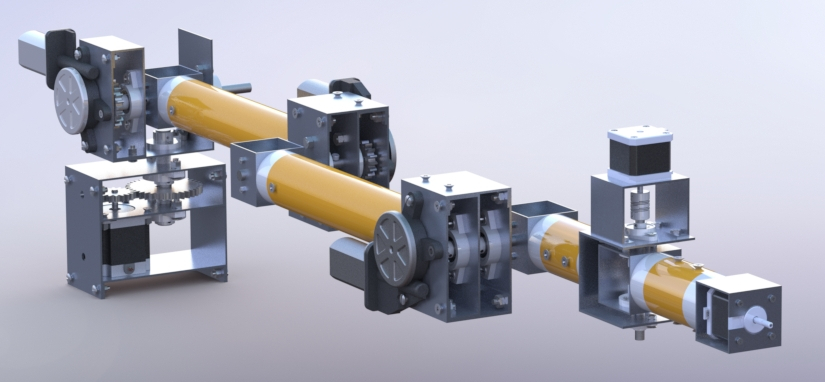
\includegraphics[width=0.8\columnwidth]{images/arm/render.jpg}
    
    \par\end{centering}

    \label{fig:manipulador-render}
\end{figure}

Através de comparação entre o sistema no ambiente 3D e o arranjo de sistemas definido no projeto base,
vísivel na figura \ref{fig:DH-Base}, foi identificada a necessidade de propor um novo modelo
lógico para o sistema, com um novo conjunto de parâmetros de Denavit-Hartenberg.
Detalhes sobre a construção do novo modelo estão disponíveis no apêndice \ref{apendice-dh}.

\begin{figure}[htb]
    \caption{Arranjo de sistemas definido no projeto base \cite{fernando2019assistivo}.}    
    \begin{centering}

        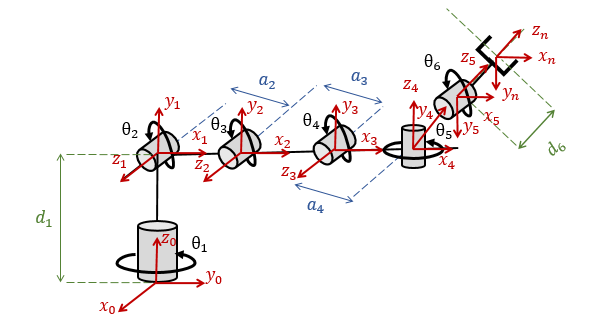
\includegraphics[width=0.8\columnwidth]{images/arm/Refframes-original.png}
    
    \par\end{centering}

    \label{fig:DH-Base}
\end{figure}

Após o posicionamento dos sistemas de referência, foi adotado para a junta 5 
uma compensação, ou \textit{offset},
com valor constante, pois originalmente, com $\theta_5=0$, o 
último elo do sistema ficaria perpendicular ao elo precedente. A compensação
foi de exatamente $-\pi/2$, para que na nova posição 0, o manipulador esteja 
completamente alongado na horizontal, bem como na figura \ref{fig:manipulador-render}.
O novo modelo desenvolvido, após inclusão desta compensação, pode ser visto na figura \ref{fig:DH-Novo}. 

\begin{figure}[htb]
    \caption{Novo arranjo de sistemas.}    
    \begin{centering}

        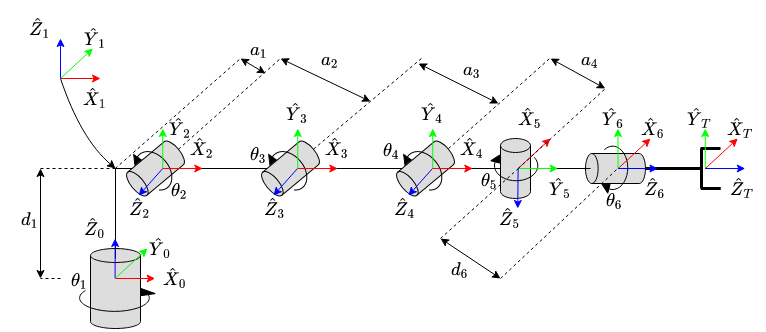
\includegraphics[width=0.8\columnwidth]{images/arm/RefFrames.png}
    
    \par\end{centering}

    \label{fig:DH-Novo}
\end{figure}

Na figura \ref{fig:DH-Novo} estão dispostos também os sistemas de referência
para a base e para a ferramenta, representados por $0$ e $T$, respectivamente.
Para a análise de torque, as transformações de base e ferramenta, $^0_1\textbf{T}$ e $^6_T\textbf{T}$,
foram assumidas como unitárias, representadas por matrizes identidade 4x4,
sem influencia sobre os resultados obtidos.

Nas imagens \ref{fig:DH-Base} e \ref{fig:DH-Novo} são visíveis os parâmetros 
comuns $d_1$, $a_2$, $a_3$, $a_4$ e $d_6$, já o parâmetro $a_1$ é exclusivo da 
nova versão. 
Esses valores são os parâmetros de DH utilizados para descrever o manipulador,
retirados do sistema montado no ambiente de modelagem 3D, como pode ser visto no
apêndice \ref{apendice-dh}. 
Uma comparação entre os dois modelos, bem como o valor dos parâmetros, pode 
ser vista na tabela \ref{tab:DH-comparacao}.

\begin{table}[htb]
    \begin{centering}

    \begin{floatrow}

    \subfloat[Modelo Origial \cite{fernando2019assistivo}.]{
        \begin{tabular}{|c|c|c|c|c|}
            \hline
            i & $\alpha_i$ &  $a_i$ (m) &  $d_i$ (m) & $\theta_i$ \\
            \hline
            \hline
            1 &   $\pi/2$  &      0     & $d_1=0,17$ & $\theta_1$ \\
            \hline
            2 &      0     & $a_2=0,35$ &      0     & $\theta_2$ \\
            \hline
            3 &      0     & $a_3=0,35$ &      0     & $\theta_3$ \\
            \hline
            4 &      0     & $a_4=0,15$ &      0     & $\theta_4$ \\
            \hline
            5 &  $-\pi/2$  &      0     &      0     & $\theta_5$ \\
            \hline
            6 &  $-\pi/2$  &      0     & $d_6=0,20$ & $\theta_6$ \\
            \hline
        \end{tabular}
    }

    \subfloat[Modelo Modificado.]{
        \begin{tabular}{|c|c|c|c|c|}
            \hline
            i & $\alpha_{i-1}$ & $a_{i-1}$ (m) &  $d_i$ (m)  & $\theta_i$ \\
            \hline
            \hline
            1 &        0       &       0       & $d_1=0.187$ & $\theta_1$ \\
            \hline
            2 &     $\pi/2$    &  $a_1=0.014$  &      0      & $\theta_2$ \\
            \hline
            3 &        0       &  $a_2=0.350$  &      0      & $\theta_3$ \\
            \hline
            4 &        0       &  $a_3=0.350$  &      0      & $\theta_4$ \\
            \hline
            5 &     $\pi/2$    &  $a_4=0.165$  &      0      & $\theta_5'$ \\
            \hline
            6 &    $-\pi/2$    &       0       & $d_6=0.198$ & $\theta_6$ \\
            \hline                                           
        \end{tabular}
    }

    \end{floatrow}

\caption{Comparação entre parâmetros DH para modelo original e modificado.}
\label{tab:DH-comparacao}

\par\end{centering}
\end{table}

É notável pela tabela \ref{tab:DH-comparacao} a diferença entre a posição dos 
parâmetros, isto ocorre pois a parte relativa ao modelo original, \ref{tab:DH-comparacao}(a),
foi representada de acordo com o observado no trabalho original, já a
parte do novo arranjo, \ref{tab:DH-comparacao}(b), foi realizada de acordo com 
a representação proposta em \cite{craig2009introduction}. Os valores encontrados para as 
constantes $a_2$ e $a_3$ foram idênticos para ambos os trabalhos, já os outros parâmetros
apresentam pequenas diferenças, inferior a 20mm, sendo estas diferenças decorrentes 
provavelmente da lógica de conexão entre as peças no ambiente de modelagem 3D. 
Na parte (b) da tabela nota-se também que a variável $\theta_5$ foi alterada 
para $\theta_5'$, representando a nova variável obtida após incluir o deslocamento 
fixo adotado nesta junta, como indica a equação \ref{eq:junta5-offset}.

\vspace{-2ex}
\begin{equation}
    \theta_5' = \theta_5 + (-\pi/2)
    \label{eq:junta5-offset}
\end{equation}

Através de ferramentas de medição disponíveis no ambiente da modelagem 3D, foram obtidos os valores de massa, tensor de inércia $\textbf{I}_T$ 
e posição do centro de massa, $\textbf{r}_{CM}$, para as juntas do sistema, os valores obtidos estão organizados na tabela \ref{tab:MrI}. 
Para melhor compreender as massas que devem ser movimentadas por 
cada junta, os sistemas foram isolados e representados nas figuras de \ref{fig:elos}(a) a \ref{fig:elos}(e).

\begin{table}[htb]
    \begin{centering}    
        
    \begin{tabular}{|c|c|c|c|}
        \hline
        Junta & $\textbf{r}_{CM}$ (3x1 m) & Massa (kg) & $\textbf{I}_T$ (3x3 kg.m$^2$) \tabularnewline
        \hline
        \hline
        1 & $\begin{bmatrix}-0,035 & -0,062 &  0,009 \end{bmatrix}^T$ & 0,674 & $\begin{bmatrix}
                                                                                    0,002 & 0,001 & 0,0     \\
                                                                                    0,001 & 0,002 & 0,0     \\
                                                                                    0,0   & 0,0   & 0,002   \\
                                                                                \end{bmatrix}$ \tabularnewline
        \hline
        2 & $\begin{bmatrix} 0,231 &  0,007 & -0,015 \end{bmatrix}^T$ & 1,257 & $\begin{bmatrix}
                                                                                    0,002 & 0,0   & -0,001  \\
                                                                                    0,0   & 0,021 & 0,0     \\
                                                                                   -0,001 & 0,0   & 0,020   \\
                                                                                \end{bmatrix}$ \tabularnewline
        \hline
        3 & $\begin{bmatrix} 0,235 & -0,008 &  0,090 \end{bmatrix}^T$ & 1,235 & $\begin{bmatrix}
                                                                                    0,002 & 0,0   & 0,002   \\
                                                                                    0,0   & 0,019 & 0,0     \\
                                                                                    0,002 & 0,0   & 0,019   \\
                                                                                \end{bmatrix}$ \tabularnewline
        \hline
        4 & $\begin{bmatrix} 0,097 &  0,030 &  0,005 \end{bmatrix}^T$ & 0,672 & $\begin{bmatrix}
                                                                                    0,002 & 0,001 & 0,0     \\
                                                                                    0,001 & 0,003 & 0,0     \\
                                                                                    0,0   & 0,0   & 0,005   \\
                                                                                \end{bmatrix}$ \tabularnewline
        \hline
        5 & $\begin{bmatrix} 0,0   &  0,091 & 0,0    \end{bmatrix}^T$ & 0,537 & $\begin{bmatrix}
                                                                                    0,002 & 0,0   & 0,0     \\
                                                                                    0,0   & 0,0   & 0,0     \\
                                                                                    0,0   & 0,0   & 0,002   \\
                                                                                \end{bmatrix}$ \tabularnewline
        \hline
        6 & $\begin{bmatrix} 0,0   & 0,0    & 0,0    \end{bmatrix}^T$ & 0,0   & $\begin{bmatrix}
                                                                                    0,0   & 0,0   & 0,0     \\
                                                                                    0,0   & 0,0   & 0,0     \\
                                                                                    0,0   & 0,0   & 0,0     \\
                                                                                \end{bmatrix}$ \tabularnewline
        \hline
    \end{tabular}
    
    \caption{Valores de massa, posição de centro de massa e tensor de inércia para as juntas.}
    \label{tab:MrI}
    
\par\end{centering}
\end{table}

\begin{figure}[h]
    \begin{centering}

    \begin{floatrow}

        \subfloat[Conjunto movimentado pela junta 1: Elo 1.]{
            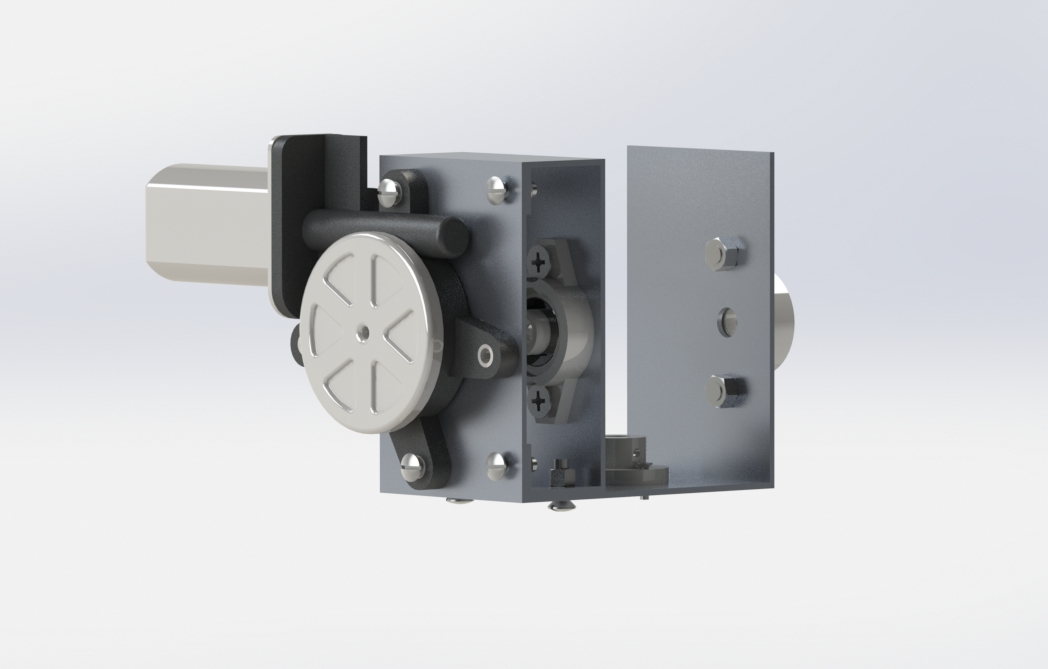
\includegraphics[width=0.4\columnwidth]{images/arm/joint1-mass-cropped.jpg}
        }

        \subfloat[Conjunto movimentado pela junta 2: Elo 2.]{
            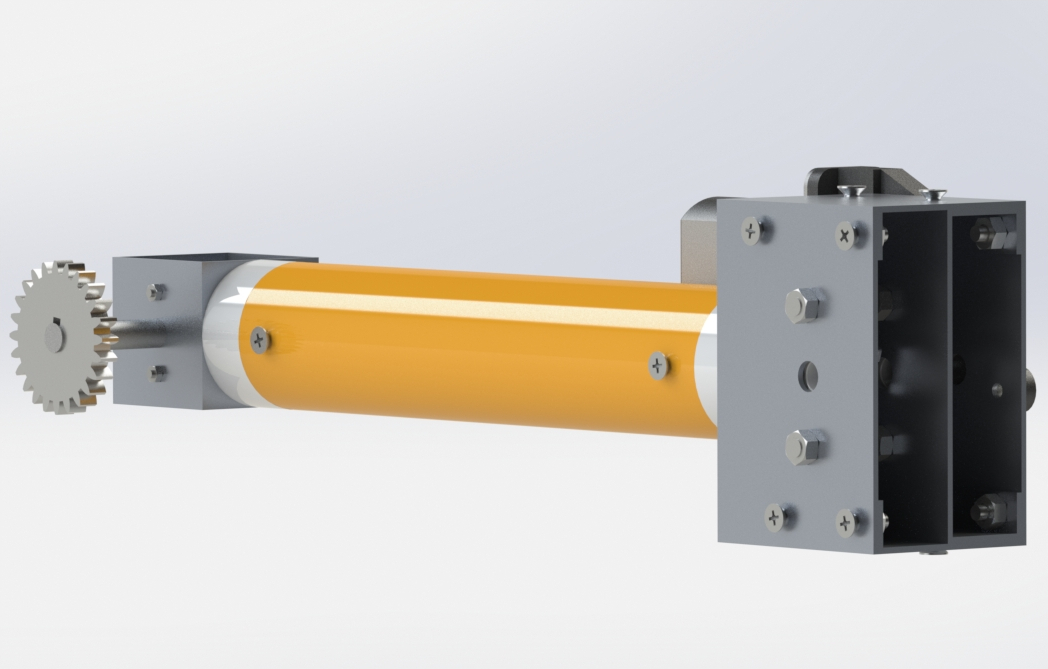
\includegraphics[width=0.4\columnwidth]{images/arm/joint2-mass-cropped.jpg}
        }

    \end{floatrow}

    \begin{floatrow}

        \subfloat[Conjunto movimentado pela junta 3: Elo 3.]{
            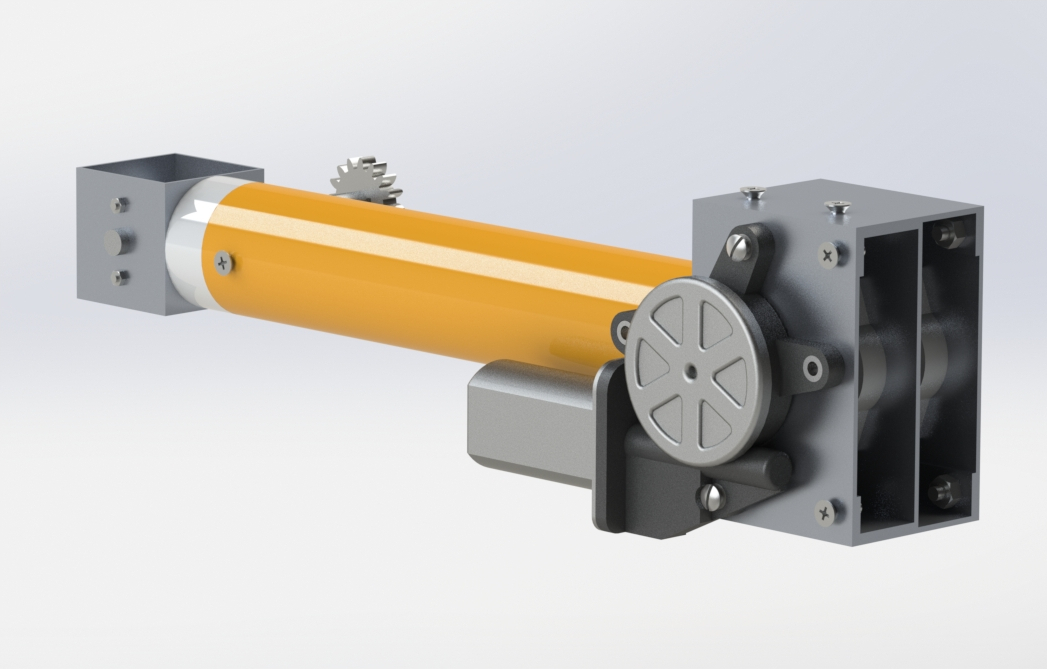
\includegraphics[width=0.4\columnwidth]{images/arm/joint3-mass-cropped.jpg}
        }
    
        \subfloat[Conjunto movimentado pela junta 4: Elo 4.]{
            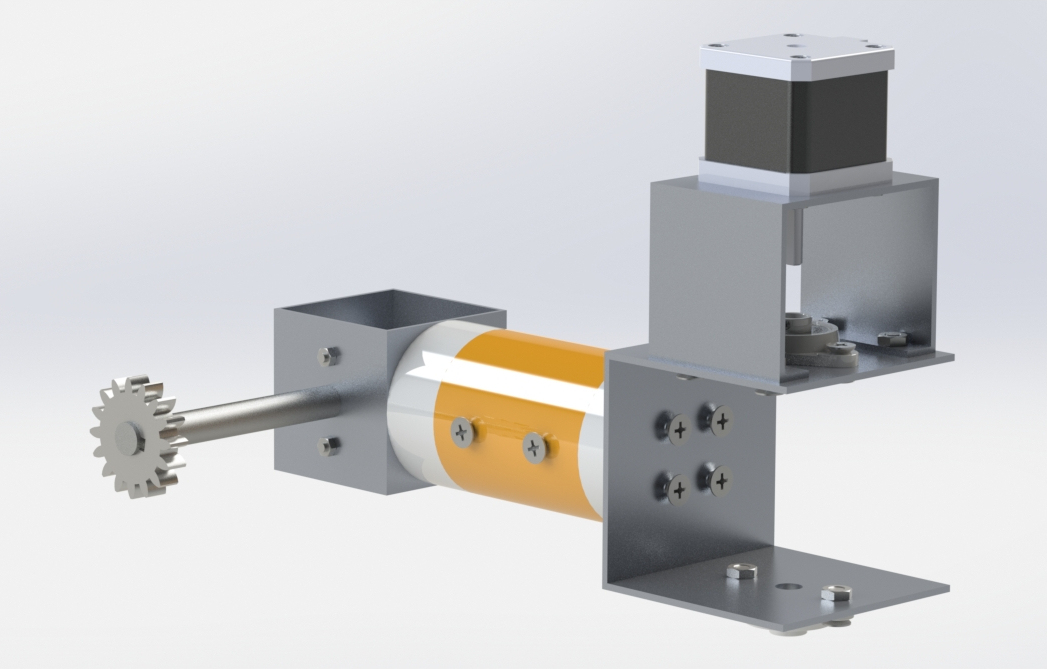
\includegraphics[width=0.4\columnwidth]{images/arm/joint4-mass-cropped.jpg}
        }
    
    \end{floatrow}

    \subfloat[Conjunto movimentado pela junta 5: Elo 5.]{
        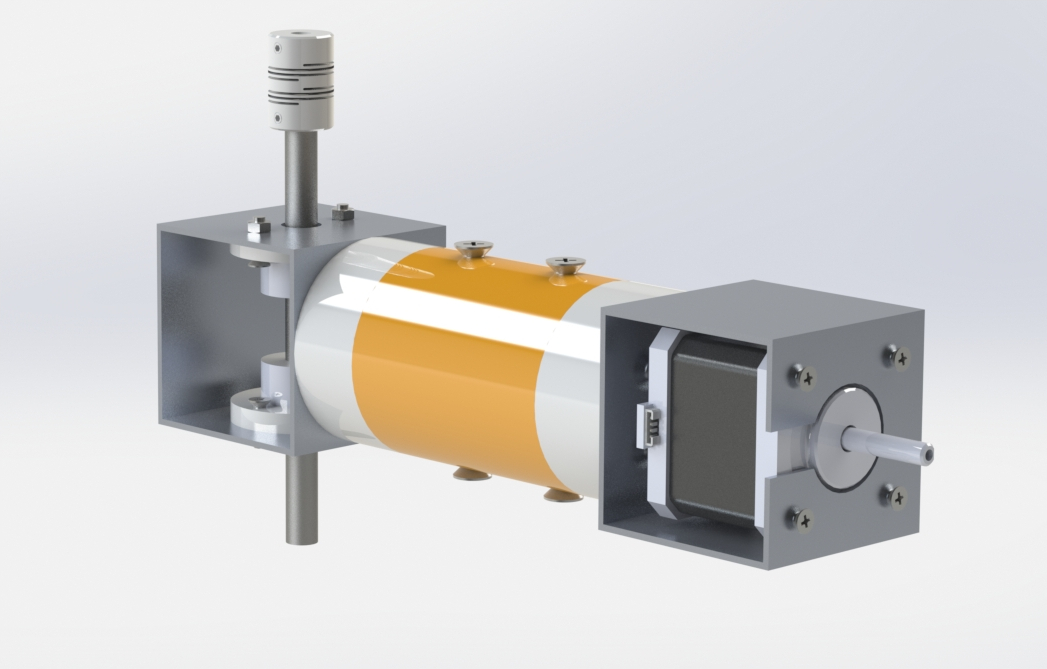
\includegraphics[width=0.4\columnwidth]{images/arm/joint5-mass-cropped.jpg}
    }

\caption{Elos isolados do manipulador.}
\label{fig:elos}

\par\end{centering}
\end{figure}

Em relação à junta 6, o eixo de saída não está diretamente conectado a nenhum equipamento, 
portanto os valores de massa e tensor de inércia são nulos, como demonstra a tabela
\ref{tab:MrI}. A ideia é que seja possível acoplar diferentes atuadores neste eixo de
saída, para uma maior adaptação do braço com o usuário e ambiente. A fim de incluir o 
efeito da carga sobre o manipulador, com o intuito de calcular o torque nas juntas, 
assumiu-se uma massa de 1,2kg a 10cm de distância do eixo de saída, e para o efeito
da gravidade, foi adotada uma aceleração vertical orientada para cima com o valor
de 9,81m/s$^2$, como indicado em \cite{craig2009introduction}.

Para a utilização das equações de Newton-Euler, se faz necessário identificar os
valores de posição, velocidade e aceleração para cada junta. Nota-se que a posição que
oferece maior resistência ao movimento para as juntas 2, 3 e 4 é aquela com as juntas 
conseguintes completamente estendidas, ampliando o efeito de braço de alavanca sobre a 
junta a ser analisada. A configuração 0, como ilustrado na imagem \ref{fig:manipulador-render}, 
maximiza a inércia observada pela junta 1, e também garante o efeito desejado para as 
juntas de 2 a 4.

O valor máximo de torque para a junta 5 pode ser observado com alguma configuração onde
a soma dos ângulos das juntas 2, 3 e 4 seja igual a 90\textdegree \, ($\theta_2+\theta_3+\theta_4=\pi/2$),
mantendo o eixo $\hat{Z}_5$ na horizontal, e o ângulo desta junta seja $\pm \pi/2$, ou seja, 
com a junta agindo contra o efeito da gravidade e maior braço de alavanca possível. Um exemplo de
configuração com estas características pode ser visto na figura \ref{fig:configuracao2}.

\begin{figure}[ht!]
    \caption{Posição do manipulador para maximização do efeito de gravidade sobre a junta 5.}    
    \begin{centering}

        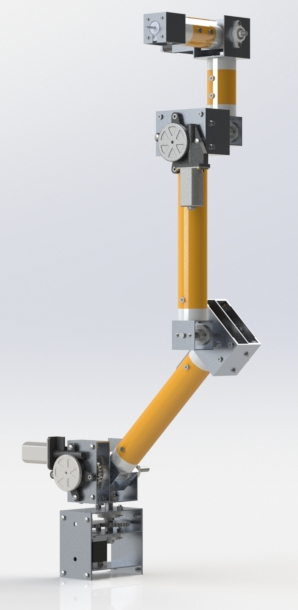
\includegraphics[width=0.2\columnwidth]{images/arm/p90.jpg}
    
    \par\end{centering}

    \label{fig:configuracao2}
\end{figure}

Todas estas informações foram agrupadas e inseridas no módulo desenvolvido para aplicação 
das equações de Newton-Euler. Foram então realizadas duas execuções, uma para a configuração 0
e outra para $\theta_2 = \pi/2$, $\theta_5 = -\pi/2$ e demais ângulos 0. Foi adotada uma 
velocidade de 0,0 rad/s e aceleração de 0,07 rad/s$^2$ para todas as juntas, seguindo a proposta
inicial do trabalho base. Os maiores valores observados foram anotados na tabela 
\ref{tab:Torques-Novo}. 

\begin{table}[htb]
    \begin{centering}    
    
    \caption{Torques recalculados, para movimento das juntas.}
    
    \begin{tabular}{|c|c|}
        \hline
        Junta & Torque calculado (N.m) \tabularnewline
        \hline
        \hline
        1 & 0,19 \tabularnewline
        \hline
        2 & 34,32 \tabularnewline
        \hline
        3 & 18,81 \tabularnewline
        \hline
        4 & 7,56 \tabularnewline
        \hline
        5 & 4,01 \tabularnewline
        \hline
        6 & 0,0  \tabularnewline
        \hline
    \end{tabular}
    
    \label{tab:Torques-Novo}
    
\par\end{centering}
\end{table}

É visível uma diferença entre a tabela dos resultados obtidos, \ref{tab:Torques-Novo}, e a tabela original dos torques 
\ref{tab:Torques}, decorrente possivelmente da diferença dos valores utilizados de massa e 
afins em cada projeto. As maiores diferenças encontradas foram nas juntas 1, 2 e 5. A diferença para a 
junta 1 pode ser explicada pelo uso da massa completa da junta 1 no trabalho base, incluindo-se no cálculo
do torque até mesmo componentes estáticos, que não são movimentados pelo eixo da junta, fato que, somando-se à 
diferenças no parâmetro $d_1$, resulta na diferença observada. Para a junta 2
a diferença pode ser atribuída a diferentes valores de massa fornecidos pelo ambiente de
modelagem 3D, já para a junta 5, o alto valor de torque provém do uso da segunda configuração de 
execução das equações de Newton-Euler.

Como algumas juntas necessitam de um torque elevado, foram utilizados pares de 
engrenagens para reduzir o esforço de atuação necessário e permitir a utilização
de motores de dimensões mais reduzidas. As relações utilizadas e os torques 
resultantes estão dispostos na tabela \ref{tab:TorquesReducao}. 

\begin{table}[h]
\begin{centering}    
    
\begin{tabular}{|c|c|c|c|c|c|c|}
    \hline
    Junta & 1 & 2 & 3 & 4 & 5 & 6 \tabularnewline
    \hline
    Redução & 1:2 & 1:3 & 1:2 & 1:2 & 1:1 & 1:1 \tabularnewline
    \hline
\end{tabular}

\caption{Redução empregada nas juntas.}
\label{tab:TorquesReducao}

\par\end{centering}
\end{table}

Para os novos valores encontrados de torque, alguns conjuntos de atuadores
e caixas de engrenagens não se mostram adequados para movimentar corretamente
o manipulador, devendo a revisão de seleção dos atuadores levar também em 
consideração uma possível modificação nas relações de engrenages utilizadas.

No que diz respeito à velocidade linear máxima para o efetuador final, 
esta foi definida para a construção do braço como sendo 15cm/s \cite{fernando2019assistivo}.
É importante notar que o alcance, ou não, desta velocidade, depende de 
fatores que influenciam as velocidades das juntas, como saturação e
posições de singularidades.

Outra informação de extrema importância para a seleção dos elementos atuadores e 
sensores pode ser retirada do projeto mecânico do manipulador, trata-se do 
deslocamento angular permitido para as juntas. Os valores de 
posicionamento máximo e mínimo para cada junta podem ser vistos na 
tabela \ref{tab:Tabela-Alcance}.

\begin{table}[h]
\begin{centering}    
    
\begin{tabular}{|c|c|c|c|c|c|c|}
    \hline
    & $\theta_1$ & $\theta_2$ & $\theta_3$ & $\theta_4$ & $\theta_5$ & $\theta_6$ \tabularnewline
    & (Base) & (Ombro) & (Cotovelo) & (\textit{Pitch}) & (\textit{Yaw}) & (\textit{Roll}) \tabularnewline
    \hline
    \hline
    Limite Angular & $\pm$90º & -45º a +135º & -135º a +160º & $\pm$160º & $\pm$90º & $\pm$360º\tabularnewline
    \hline
\end{tabular}
    
\caption{Limites de movimentação para as juntas.}
\label{tab:Tabela-Alcance}

\par\end{centering}
\end{table}

Os valores contidos na tabela \ref{tab:Tabela-Alcance} ditam os limites 
de leitura que devem ser obtidos através dos equipamentos de medição a 
serem aplicados, de tal modo que a precisão obtida seja suficiente 
para um posicionamento fino de cada junta nos valores intermediários.

\section{Análise e Seleção}
\label{sec:AnaliseEletro}

% Aceleracao em relacao a selecao de atuadores

\subsection{Atuadores}

Como já descrito, o robô base conta com um conjunto de atuadores 
previstos para o seu funcionamento, portanto, com base nos valores 
apresentados, este conjunto deve ser revisado juntamente com outras 
possibilidade de atuadores e resultar ao final na seleção de elementos 
capazes de movimentar o braço robótico pautando-se nas especificações 
escolhidas, sendo estas: 

\begin{itemize}
    \item Torque máximo;
    \item Potência consumida;
    \item Precisão;
    \item Massa introduzida no sistema;
    \item Facilidade de inclusão na estrutura mecânica;
    \item Método de acionamento;
    \item Preço;
    \item Durabilidade.
\end{itemize}

O torque máximo e potência consumida são fatores limitantes na escolha de atuadores
para um projeto robótico, devendo estes serem respeitados para que o robô possa
se movimentar como desejado. Já o critério de precisão é um fator de interesse 
quando se deseja que o produto desenvolvido apresente capacidade de repetibilidade e 
confiança na movimentação, sendo portanto um fator a ser considerado neste projeto.

A massa dos atuadores escolhidos é de extrema importância para evitar sobrecarregar 
outras partes do sistema. De maneira semelhante, o critério de facilidade 
de inserção analisa como se dará a junção dos atuadores à estrutura do 
braço e à cadeira de rodas. O método de acionamento deve ser observado 
para evitar introduzir no sistema um alto grau de complexidade em relação 
ao circuito de acionamento. O preço e a durabilidade são dois parâmetros 
importantes nesse projeto, sendo estes os fatores desejados para incorporar
um diferencial ao produto desenvolvido quando comparado a outras alternativas.

Partindo do critério sobre a facilidade de inclusão de atuadores ao sistema, 
é interessante considerar também o local de aplicação do braço mecânico, 
para que sejam escolhidos atuadores que possuam maior aderência com o 
sistema como um todo. 
Uma comparação foi realizada em \cite{fernando2019assistivo} entre as 
opções de uso de atuadores elétricos, hidráulicos e pneumáticos, bem como
entre atuação direta e indireta. O autor, por fim, optou pelo uso de 
atuadores elétricos e método de acionamento direto, garantindo um projeto
mais compacto como um todo.

No entanto, dentre as desvantagens apresentadas pelo autor
para o método de atuação direta, está o baixo torque de atuação, que acaba
se tornando um problema quando são comparadas as tabelas \ref{tab:Motores},
\ref{tab:Torques-Novo} e \ref{tab:TorquesReducao}, onde os conjuntos 
atuador/caixa de redução empregados nestas juntas não se mostram capazes
de movimentar corretamente o robô. Esta análise está simplificada na 
tabela \ref{tab:Analise-Torque}.

\begin{table}[htb]
    \begin{centering}    
    
    \caption{Torques fornecidos e necessários para movimento das juntas.}
    
    \begin{tabular}{|c|c|c|c|c|}
        \hline
        Junta & Torque motor (N.m) & Redução & Torque resultante (N.m) & Torque necessário (N.m) \tabularnewline
        \hline
        \hline
        1 & 1,25 & 1:2 &  2,50 &  0,19              \tabularnewline
        \hline
        2 & 9,12 & 1:3 & 27,36 & \color{red}{34,32} \tabularnewline
        \hline
        3 & 9,12 & 1:2 & 18,24 & \color{red}{18,81} \tabularnewline
        \hline
        4 & 9,12 & 1:2 & 18,24 & 7,56               \tabularnewline
        \hline
        5 & 0,43 & 1:1 &  0,43 & \color{red}{4,01}  \tabularnewline
        \hline
        6 & 0,43 & 1:1 &  0,43 & 0,0                \tabularnewline
        \hline
    \end{tabular}
    
    \label{tab:Analise-Torque}
    
\par\end{centering}
\end{table}

A compacidade apontada como vantagem do modo de atuação direto acaba
se tornando então uma desvantagem neste projeto, pois, devido ao método
de construção das juntas, a troca de atuadores se mostra trabalhosa,
bem como inserção de elementos externos para compensar o baixo torque dos atuadores.
A figura \ref{fig:mola} ilustra uma tentativa de inserção de mola na 
estrutura, para compensar o baixo torque do atuador na junta 2 do sistema.

\begin{figure}[h!]
    \caption{Inclusão de mola para compensação de torque na junta 2.}    
    \begin{centering}

        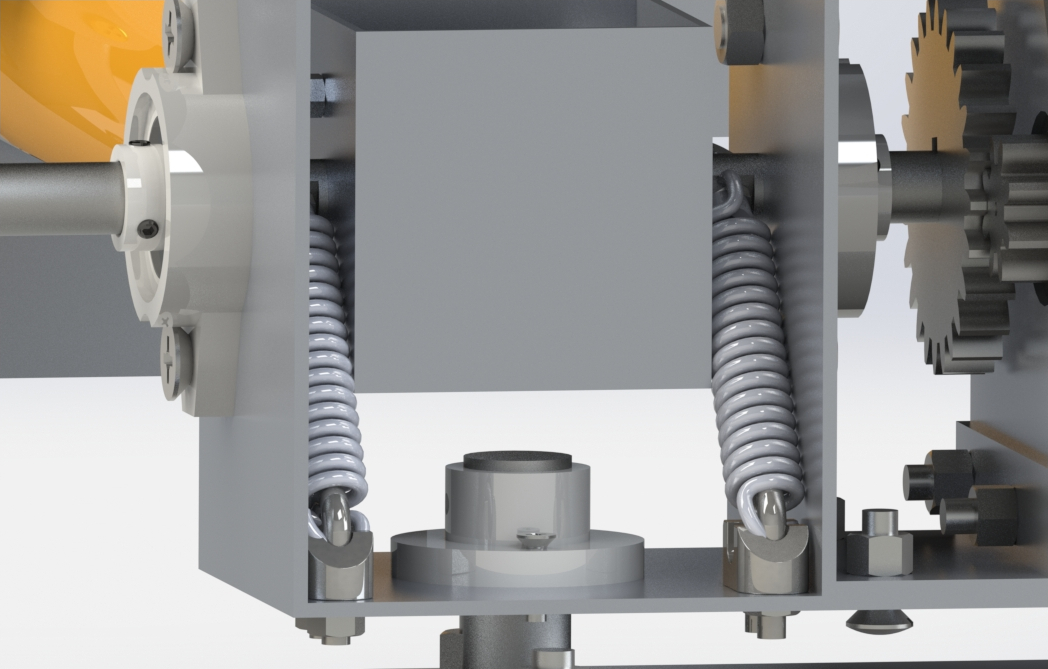
\includegraphics[width=0.7\columnwidth]{images/arm/spring-cropped.jpg}
    
    \par\end{centering}

    \label{fig:mola}
\end{figure}

Para aplicação da mola de acordo com a figura \ref{fig:mola}, seria necessário
usinar o eixo de rotação do elo, bem como modificar a própria estrutura da junta, 
implicando em mudanças na resistência mecânica desta. A mola necessitaria ainda
de um valor de constante relativamente alto para uma boa compensação, portanto 
esta opção foi descartada.

A opção mais simples encontrada para resolver o problema de falta de torque nos
atuadores foi a alteração da relação de engrenagens aplicadas 
nestas juntas. As juntas 2 e 3 apresentam uma distância fixa entre os centros das 
engrenagens, por isso, se fez necessário incluir um adaptador para a saída dos 
motores Mabuchi, modificando a relação nestas juntas para, respectivamente, 1:4,5 e 
1:2,5. A junta 5 é a que apresenta maior espaço para modificações, fornecendo maior 
liberdade para aplicar uma relação de engrenages contínua, ou uma caixa de engrenagens
planetária, sendo necessário que a redução final seja no mínimo de 1:10.

A mudança nestas relações fornece ainda uma melhora na precisão de atuação destas 
juntas, redução da potência elétrica consumida através da redução do torque e, 
consequentemente, potência mecânica requerida e ao mesmo tempo mantém as vantagens 
citadas pelo autor em relação ao acionamento, preço e compacidade dos equipamentos.

\subsection{Sensores}
% Expor as possibilidades de sensores dado cada escolha de atuadores para cada junta
% Potênciometro, encoder, hall, fim de curso
Em relação ao sensoriamento, é necessário que existam no manipulador 
sensores de posição angular para as juntas onde serão utilizados 
atuadores sem uma boa resposta a acionamento em malha aberta. Estes sensores
também podem ser utilizados nas juntas que empregam atuadores com 
resposta em malha aberta suficientemente confiável, buscando garantir 
um grau de redundância em relação ao posicionamento. A escolha por determinada 
classe de sensor deve se basear também no nível de adaptação necessária para 
incluí-lo no robô. 

A escolha dos elementos de sensoriamento é largamente relacionada com a 
quantidade, o modo de leitura e a aplicação destes, buscando não sobrecarregar os circuitos 
de processamento de sinais mas ainda sim garantir um bom conhecimento 
acerca do estado do braço robótico. 

Foram comparadas as possibilidades de uso de sensores digitais do tipo \textit{encoder}
e sensores potênciometros análogicos.
Os principais fatores levados em consideração foram preço, facilidade de 
inserção na estrutura do robô e resolução de leitura. 
A massa dos sensores analisados se mostrou desprezível em relação à massa dos 
atuadores e das juntas como um todo, bem como a potência consumida por 
estes, logo, estes parâmetros não foram levados em consideração para 
comparação entre os tipos de equipamentos.

Em relação à inserção na estrutura, ambas opções apresentam fatores similares, 
podendo ser conectados ao eixo de rotação das juntas. 
Um cuidado a ser tomado em relação a potenciômetros é que estes possuem uma 
faixa limitada de operação, que deve ser respeitada em sua aplicação.

Do ponto de vista da precisão, inicialmente foi realizada uma comparação entre o uso de 
um conjunto potenciômetro com conversor ADC de 10 bits, comum nas placas controladoras
Arduino, contra um \textit{encoder}.  
Seguindo a equação \ref{eq:res_adc}, o ADC forneceria uma resolução de $1/2^{10}$, o que para 
um ângulo de entrada máximo de 360\textdegree, equivaleria a aproximadamente 0,35\textdegree.
Para que esse valor seja respeitado, é importante escolher um potenciômetro com boa resolução, 
como um potenciômetro de precisão.
Para obter a mesma resolução utilizando um \textit{encoder}, seria necessário que o mesmo emitisse
por volta de 1020 pulsos por revolução, de acordo com a equação \ref{eq:res_encoder}.

Partindo dos dados apresentados, somando-se aos fatos de que \textit{encoders} com 
um valor de $PPR$ próximo ao apontado apresentaram um custo elevado, e que a 
inclusão de engrenagens com um alto fator de transmissão para permitir o uso 
de \textit{encoders} com uma menor resolução seria trabalhoso, optou-se pelo
uso de potenciômetros de precisão para medição da posição das juntas.

Dada a angulação máxima das juntas de acordo com a tabela 
\ref{tab:Tabela-Alcance} e o fato de que grande parte dos potênciometros 
comerciais são limitados a uma rotação máxima de 300º, optou-se por 
utilizar potenciômetros de precisão multi-voltas, que atenderia aos 
requisitos de angulação mínima e máxima de todas as juntas.

Um potenciômetro encontrado que atende aos requisitos apresentados foi o da 
família \textit{Bourns 3590}, que apresentou também um preço acessível e 
uma boa resolução, na casa de 0,02\% da tensão de saída desejada. Para confirmar
esta resolução indicada na sua ficha catalográfica, foi realizado um experimento, 
que consistiu em utilizar um \textit{laser} e um espelho conectado a um sensor 
deste tipo. O raio de luz emitido pelo \textit{laser} foi direcionado até o 
espelho, e a distância $d$ percorrida pelo raio refletido foi medida, causada por 
uma rotação no sensor potenciômetro conectado ao espelho. 
Uma ilustração do experimento pode ser vista na figura \ref{fig:teste-pot}. 
Os resultados obtidos serão discutidos na seção de resultados deste documento.

\begin{figure}[h!]
    \caption{Teste para validação da resolução do potenciômetro escolhido.}    
    \begin{centering}

        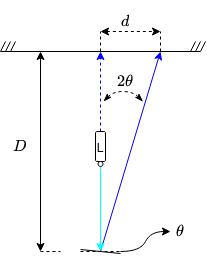
\includegraphics[width=0.3\columnwidth]{images/sensors/TestePot.png}
    
    \par\end{centering}

    \label{fig:teste-pot}
\end{figure}

Na figura \ref{fig:teste-pot} o raio na cor ciano indica o raio gerado pelo \textit{laser} L e que
chega ao conjunto espelho/potenciômetro, e 
os raios azuis-escuro indicam os raios refletidos pelo espelho, inicialmente com o espelho 
perpendicular ao raio de luz, raio tracejado, e após o sensor ser rotacionado manualmente o menor ângulo $\theta$
possível detectado por um microcontrolador Arduino. Medindo os valores de $d$ e $D$, é possível calcular a 
rotação do sensor através da equação \ref{eq:teste-pot}. Este valor de rotação, por ser equivalente ao 
menor valor detectável na saída, equivale à resolução do conjunto potenciômetro/ADC de 10 bits.

\begin{equation}
    \label{eq:teste-pot}
    \theta = \frac{tan^{-1}\left(\frac{d}{D}\right)}{2}
\end{equation}

%Falar da relação de engrenages

Verificada a resolução indicada para o potenciômetro, foram selecionados 3 potênciometros de 
precisão multi-voltas para as juntas 2, 3 e 4, que não possuem uma boa resposta em malha 
aberta.

Embora os sensores potenciômetros já permitam um conhecimento acerca 
da posição absoluta das juntas, serão ainda incluidos nessas juntas 
sensores fim-de-curso, buscando atingir um maior nível de confiabilidade e 
segurança no sensoriamento. 
Sensores desse tipo também serão aplicados nas outras juntas, onde, 
juntamente com a boa resposta em malha aberta dos motores de passo, 
espera-se obter um bom conhecimento geral sobre o posicionamento do 
manipulador robótico. Para cada junta serão inseridos dois sensores fim-de-curso,
para localizar os pontos de máxima e mínima rotação, com exceção na junta 6,
que permite rotação contínua, será utilizado apenas um único sensor, 
para referenciar o ponto zero da junta.

\subsection{Circuitos de potência}
Para análise dos circuitos de acionamento a serem empregados, foram utilizados como 
critérios de escolha principais a tensão e corrente de trabalho do 
circuito, a fim de garantir que a potência elétrica demandada pelos 
atuadores seja satisfeita, além do custo de aquisição e fatores de proteção 
empregados.

% Drivers a comparar:
%   - Dual VNH5019
%   - BTS7960
%   - MD30C
%   - BTN7971

No caso dos motores DC de rotação contínua optou-se pela utilização de 
circuitos do tipo ponte H, dada a sua boa capacidade de ativação deste 
tipo de motor, disponibilidade no mercado e segurança de aplicação. Os 
circuitos integrados VNH5019, BTS7960, MD30C e BTN7971B são exemplos de 
circuitos de acionamento comerciais utilizados para o controle de velocidade de 
motores DC que fazem uso desta tecnologia. 
Sendo um circuito de baixo custo, confiável e capaz de 
fornecer a corrente requisitada pelos motores DC selecionados, a escolha 
pelo circuito BTS7960 é favorecida frente ao projeto de um novo circuito 
ou outros modelos comerciais, logo, este circuito será o empregado no 
manipulador para o controle dos motores DC. 

Em relação à ativação das bobinas dos motores de passo, os circuitos 
comerciais L298N, DRV8825, A4988 e TB6560 são exemplos de circuitos de acionamento
comumente empregados, e para a aplicação em questão, notou-se que o mais indicado seria 
o DRV8825, sendo capaz de oferecer até 2.5A para a alimentação de motores 
de passo, além de apresentar um baixo custo e possibilidade de utilizar
diversas configurações de passo, como passo completo ou 1/32 micro-passo. 

Desse modo, serão utilizados 3 circuitos do tipo BTS7960 e 3 circuitos do 
tipo DRV8825, caracterizando ainda uma aplicação de baixo custo, frente a 
outras tecnologias semelhantes.

\subsection{Circuitos de processamento de sinal e comando}

Os quesitos a serem atendidos pelo circuito principal de processamento são: 
capacidade de leitura de todos os sensores propostos, capacidade de 
controlar a ativação dos atuadores propostos, capacidade de controle 
embarcado, facilidade de programação e, por fim, custo.

Além dos sensores de posição já citados, é necessário também preparar o 
sistema de processamento e comando para incluir algum equipamento que realizará
a tradução dos comandos do operador para comandos de movimentação da estrutura.
Para este projeto, adotou-se que a interação com o usuário será realizada por 
meio de um \textit{joystick}, técnica de interface comum a WMRAs.
O \textit{joystick} escolhido foi o modelo KY-023, 
com dois eixos de movimentação contínua e um eixo discreto, 
equivalente a dois potenciômetros perpendiculares e um botão. Este modelo 
foi escolhido por apresentar uma interface de conexão simples e baixo custo,
fatores que permitiriam uma troca futura por algum outro equipamento semelhante.

Levando em consideração então os 3 sensores potenciômetros, os 11 sensores 
fim-de-curso e o \textit{joystick}, seriam necessárias no controlador subjacente 
5 entradas analógicas e 12 entradas digitais. 
Em relação aos circuitos de potência, cada dispositivo BTS7960 necessita de um 
mínimo de 2 pinos digitais que permitam funcionalidade PWM, 
já o dispositivo DRV8825 necessita de no mínimo 2 pinos digitais, onde estes pinos 
representam os sinais de direção e avanço do motor controlado. 
Optou-se também por utilizar um pino extra nestes circuitos integrados que permite 
desligar o circuito quando este não estiver demandando um alto torque, poupando energia do sistema. 
Desse modo, ao total serão necessários no mínimo 5 entradas 
analógicas, 12 entradas digitais e 15 saídas digitais,
dessas, no mínimo 6 devem apresentar funcionalidade PWM.  

O processador ATmega-2560 foi escolhido como unidade de processamento 
primária para o manipulador por apresentar interfaces suficientes para 
os periféricos propostos, além de um baixo custo. A placa comercial 
`Arduino Mega', que utiliza este processador, se mostra como uma possível 
solução geral a ser aplicada como controladora do manipular, por ser 
acessível, ser \textit{open-source}, e já estar bem solidificada no mercado. 
Esta placa possui 54 portas digitais, das quais 15 apresentam funcionalidade 
PWM, 16 portas analógicas, velocidade 
de processador de 16Mhz e um ambiente de programação próprio que aceita a 
linguagem de progração C++. Dadas estas características, nota-se que esta 
opção é mais do que suficiente para o problema em questão, permitindo ainda 
melhorias futuras e inserção de uma maior quantidade de elementos de 
sensoriamento e atuação, logo, esta será empregada como unidade microcontroladora
(MCU) para todo o robô.

Para o tratamento dos dados provenientes dos sensores empregados serão 
utilizados componentes como resistores, capacitores e amplificadores 
operacionais, organizados de modo a garantir uma boa filtragem e condicionamento 
das leituras do robô, bem como optoacopladores, para garantir maior segurança no envio
de sinais elétricos.
As topologias empregadas serão discutidas nas seções seguintes.

\section{Placas de sensoriamento}

Em relação às placas de sensoriamento, que realizam o tratamento inicial 
do sinais de leitura dos sensores, foi adotado que estas deveriam 
ser posicionadas o mais próximo possível do local de leitura,
evitando o envio do sinal em sua forma bruta por cabos longos, mitigando
possíveis interferências sobre o sinal. Embora haja uma diferença na quantidade
e tipo de sensores utilizados em cada junta, optou-se por utilizar a mesma
placa em todas as juntas, buscando facilitar os processos de projeto, manufatura
e principalmente possíveis reposições. As placas serão diferenciadas entre si 
pela quantidade de equipamentos devidamente montados, ou soldados, na mesma, não
sendo necessário incluir todos os dispositivos em uma placa, a depender da junta
onde esta será aplicada.

As dimensões máximas possíveis para as placas deste tipo foram retiradas 
do espaço diponível para acoplamento nas juntas. A figura \ref{fig:dimensoes-pcb1} 
agrupa as restrições de tamanho impostas sobre o tamanho possível das placas. 

\begin{figure}[ht!]
    \begin{centering}

    \begin{floatrow}

        \subfloat[Dimensões disponíveis nas juntas 3 e 4.]{
            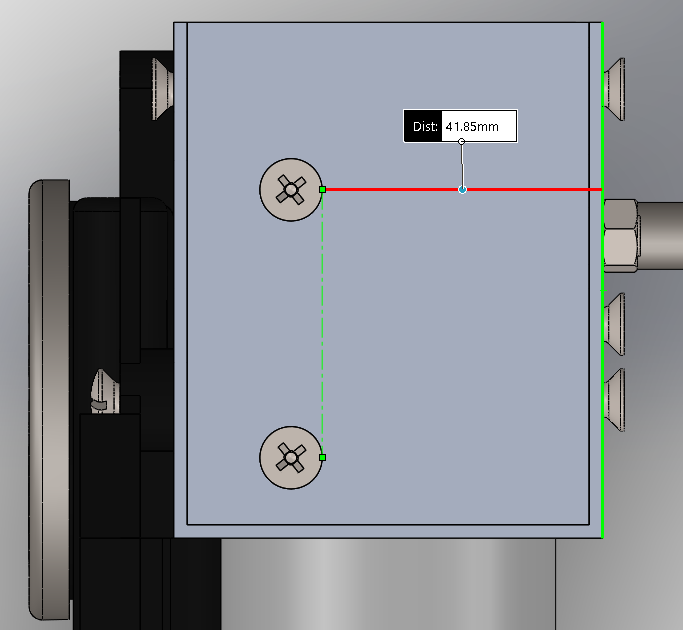
\includegraphics[width=0.5\columnwidth]{images/pcbs/SensorPCB-SizeConstraints2.png}
        }

        \subfloat[Dimensões disponíveis nas juntas 5 e 6.]{
            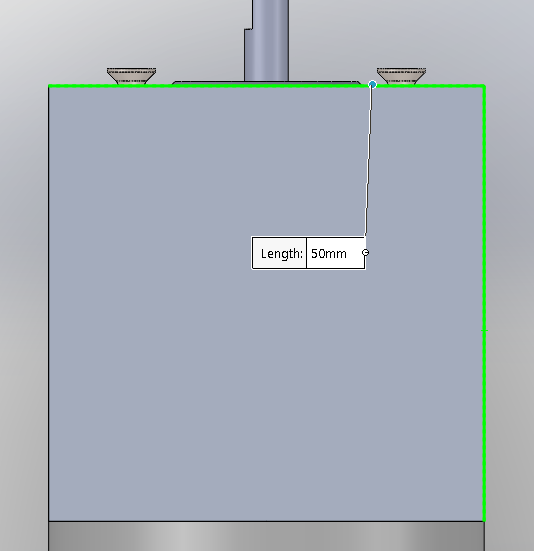
\includegraphics[width=0.45\columnwidth]{images/pcbs/SensorPCB-SizeConstraints3.png}
        }

    \end{floatrow}

    \subfloat[Dimensões disponíveis na junta 2.]{
        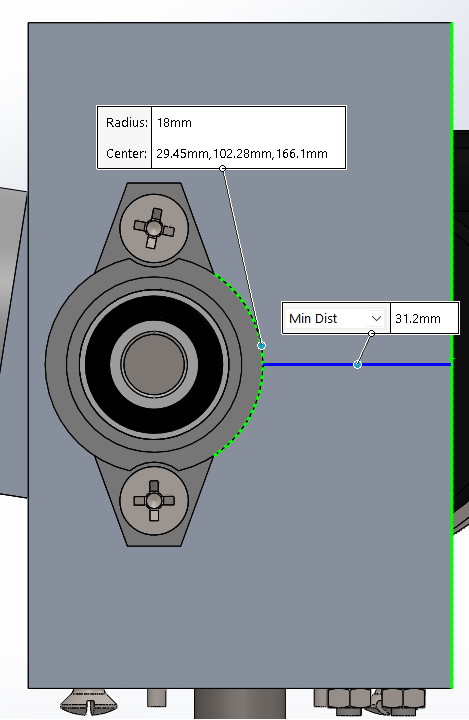
\includegraphics[width=0.5\columnwidth]{images/pcbs/SensorPCB-SizeConstraints1.png}
    }

\caption{Dimensões para inserção de placa nas juntas.}
\label{fig:dimensoes-pcb1}

\par\end{centering}
\end{figure}

Analisando as diversas limitações de tamanho nas juntas, optou-se
por projetar uma placa de dimensões 45x30mm, sendo o lado de 30mm escolhido
para respeitar o limite de 31.2mm na junta 2 e o valor de 45mm utilizado para 
respeitar os limites das outras juntas, mas ainda garantindo um bom espaço para
o projeto do circuito.
A área obtida para o projeto do circuito a ser gravado na placa foi um fator
limitante na escolha dos tipos de componentes a serem empregados, pois 
componentes \textit{through-hole} e seus furos, por utilizaram uma grande área, 
tornariam o projeto ainda mais difícil, mesmo em uma placa dupla face.

As placas de sensoriamento foram dividas em três circuitos: circuito regulador
de tensão, circuito de condicionamento do sinal analógico do potenciômetro e 
circuito de condicionamento dos sinais de sensores fim-de-curso. O circuito 
regulador de tensão foi empregado buscando-se manter os dados de leitura o
mais próximo possível do nível de segurança permitido para entrada no 
microcontrolador. O componente regulador de tensão escolhido foi o AMS-1117, 
modelo com 5V de saída e tipo SOT-223. Em conjunto com o regulador, foram
aplicados capacitores de desacoplamento, ambos de tântalo com valores de 
10uF, sendo posicionados o mais próximo possível da placa, seguindo as
recomendações do fabricante, na ficha catalográfica do dispositivo.

Na figura \ref{fig:Esquematico-regulador} são visíveis os dois capacitores
de desacoplamento no circuito regulador, sendo utilizados para filtrar
as tensões de entrada e saída e aumentar a estabilidade do circuito integrado
(CI) regulador. Para funcionamento correto do regulador, é necessário que 
a tensão de entrada supere a queda de tensão do equipamento, com valor máximo de 1.3V, de
acordo com a ficha catalográfica. A tensão de 12V da bateria escolhida é suficiente
para esta finalidade, ainda estando dentro do nível de segurança de 15V informado
para o dispositivo.

\begin{figure}[h]
    \caption{Esquemático de regulação de tensão das placas de sensoriamento}    
    \begin{centering}

        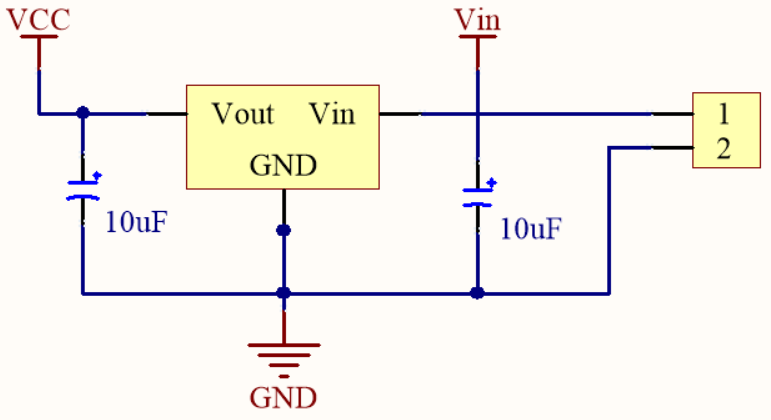
\includegraphics[width=0.5\columnwidth]{images/pcbs/SensorPCB-Regulator.png}
    
    \par\end{centering}

    \label{fig:Esquematico-regulador}
\end{figure}

Para a leitura do potenciômetro, o valor resultante da divisão de tensão 
interna é submetido a um filtro RC do tipo passa-baixas e um amplificador 
operacional não-inversor, buscando-se manter uma certa estabilidade no valor lido e uma alta
impedância de entrada no circuito condicionador, evitando influenciar a 
potência do sinal lido. Os elementos do filtro RC foram escolhidos de modo a propiciar uma 
constante de tempo para a o sistema igual a 1ms.
O ganho do amplificador é definido de modo a se obter 5V na saída para a máxima 
angulação da junta, desse modo, a variação máxima de leitura é mantida fixa.
O circuito resultando pode ser visto na figura \ref{fig:Esquematico-sensor-pot}. 

\begin{figure}[ht]
    \caption{Esquemático de leitura do potenciômetro}    
    \begin{centering}

        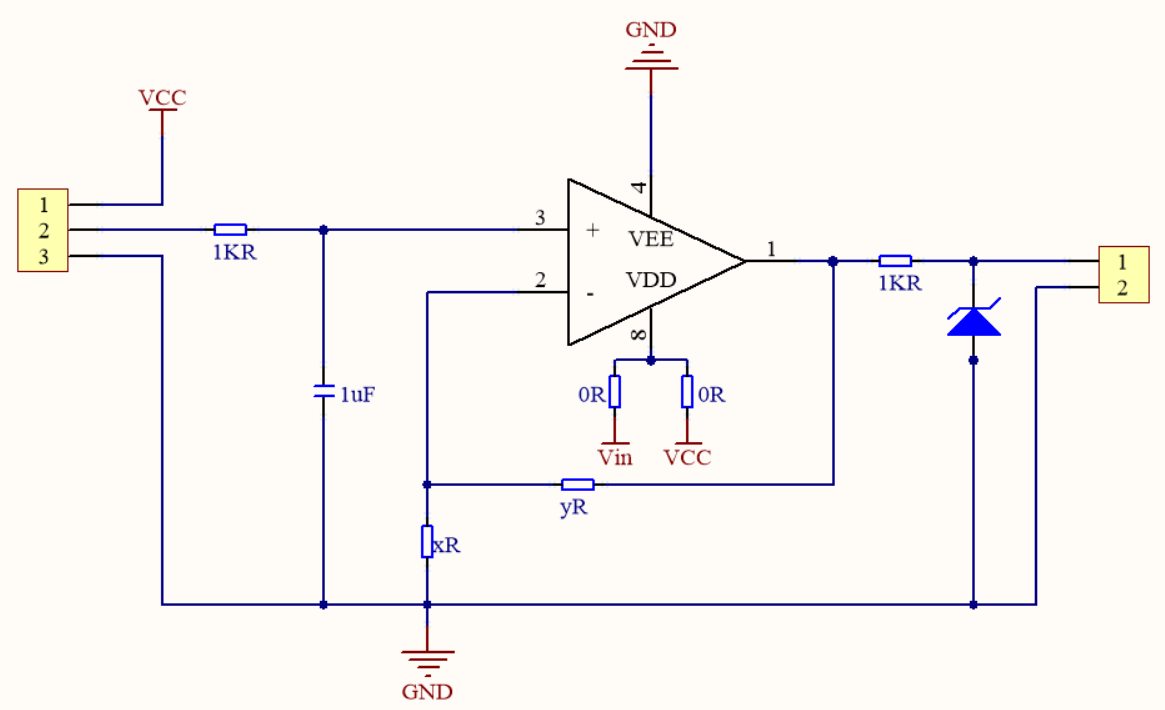
\includegraphics[width=0.75\columnwidth]{images/pcbs/SensorPCB-Pot.png}
    
    \par\end{centering}

    \label{fig:Esquematico-sensor-pot}
\end{figure}

Foi definido que o amplificador operacional empregado deve apresentar 
funcionamento do tipo \textit{Single-Supply}, de modo a simplificar
o circuito de alimentação deste.
Outra característica interessante a este amplificador seria a de apresentar
uma saída \textit{rail-to-rail}, permitindo que os valores de saída sejam 
valores próximos ao de alimentação, assim, o amplificador poderia ser 
alimentado com a mesma tensão de funcionamento das portas análogicas de leitura
do arduino, garantindo maior segurança ao sistema.
Como amplificadores deste tipo apresentaram um preço
de compra elevado, optou-se por permitir que o amplificador seja alimentado 
diretamente pela alimentação da placa ou pelo regulador de tensão empregado,
permitindo o uso tanto de amplificadores \textit{rail-to-rail} quanto aqueles
que não possuem essa característica. Estas duas possibilidades de alimentação
estão visíveis na figura \ref{fig:Esquematico-sensor-pot}, onde somente um dos 
resistores de 0R deve ser montado, indicando a tensão de entrada.

A saída do amplificador é ainda limitada a 5,1V através do uso de um resistor 
e um diodo, o resistor é empregado para evitar que a limitação seja imposta 
diretamente sobre a saída do amplificador, resultando em uma realimentação
incorreta do sistema eletrônico. O valor do resistor foi escolhido de modo
a respeitar uma dissipação de potência neste resistor de no máximo 0,05W.
Assumindo que em caso de falhas a saída do amplificador possa chegar a 12V, 
a queda de tensão no resistor seria de 6,9V. Utilizando a equação para potência 
elétrica em um resistor, chega-se a um valor mínimo de resistência de aproximadamente
950$\Omega$, o valor comercial mais próximo, de 1k$\Omega$, foi então utilizado.

O circuito inicial foi projetado utilizando o modelo para um amplificador 
operacional ideal: Impedância de entrada infinita, impedância de saída 
nula e curto virtual na entrada. A configuração não-inversora foi 
escolhida com base na alta impedância de entrada e no ganho positivo, evitando 
a necessidade de tratar tensões de valores negativos.
Para compensar as características de funcionamento não ideal dos amplificadores,
buscou-se um CI com baixa tensão de \textit{offset}, boa compensação da
corrente de \textit{bias} e uma boa taxa de rejeição de modo comum.
Com base nos dados apresentados, escolheu-se o CI LM358 para amplificação,
na sua configuração SOIC-8, por ser um circuito acessível, mas com boas
características.

Os resistores indicados com valores x e y na figura \ref{fig:Esquematico-sensor-pot}
indicam os resistores sem valor pré-definido, a serem determinados com base
em uma possível relação de engrenagens entre o eixo da junta e o sensor, para
configurar o valor máximo da leitura sempre de modo a utilizar toda 
a escala disponível de leitura no conversor ADC do microcontrolador.

Como dito anteriormente, nem todas as juntas empregam todos os circuitos projetados
na placa, sendo que este circuito do potenciômetro não será montado nas juntas 1,
5 e 6.

Para os circuitos dos sensores fim-de-curso, fez-se uso de um circuito 
RC do tipo filtro passa-baixas para tratamento do sinal. 
Foi inserido também um resistor \textit{pull-down} diretamente 
em um dos pinos de conexão do sensor, mantendo o sinal em um nível 
conhecido. O resistor \textit{pull-down} foi dimensionado também respeitando
uma potência máxima de dissipação de 0,05W.
O valor comercial de 10K foi adotado para este resistor visando reduzir a
corrente, e as perdas por efeito Joule, nesta parte do circuito, 
ainda obedecendo o valor mínimo específicado. 
Os valores dos componentes do circuito RC foram escolhidos de modo a 
facilitar a escolha por componentes comerciais. Tomando como base um 
valor para a constante de tempo próximo a 50ms, foi escolhido um valor 
para a resistência igual a 47k e 1uF para o capacitor.

Na saída do circuito RC foi inserido um amplificador operacional no 
modo seguidor de tensão, buscando desacoplar o circuito de 
interfaceamento do circuito de sensoriamento e condicionamento. 
As mesmas análises realizadas para o circuito do potenciômetro foram 
levadas em consideração no emprego deste amplificador, no entanto, por 
se tratar de um sinal analisado como digital, foi possível empregar o 
amplificador de um modo mais brando.

Os amplificadores na configuração não-inversora garantem uma alta impedância 
de leitura, funcionando apenas como um \textit{buffer} para a interface.
A saída é ainda limitada do mesmo modo como foi projetado para o sinal
analógico do potenciômetro. 
A tensão de saída é então enviada ao conector 
juntamente com um sinal de ground, para que o sinal do sensor 
fim-de-curso possa ser enviado via par de cabos trançados, buscando evitar
interferências na comunicação entre as placas.

A figura \ref{fig:Esquematico-sensor-switch} mostra os diversos
componentes utilizados no tratamento da leitura dos sensores
fim-de-curso.

\begin{figure}[ht]
    \caption{Esquemático de leitura dos sensores fim-de-curso}    
    \begin{centering}

        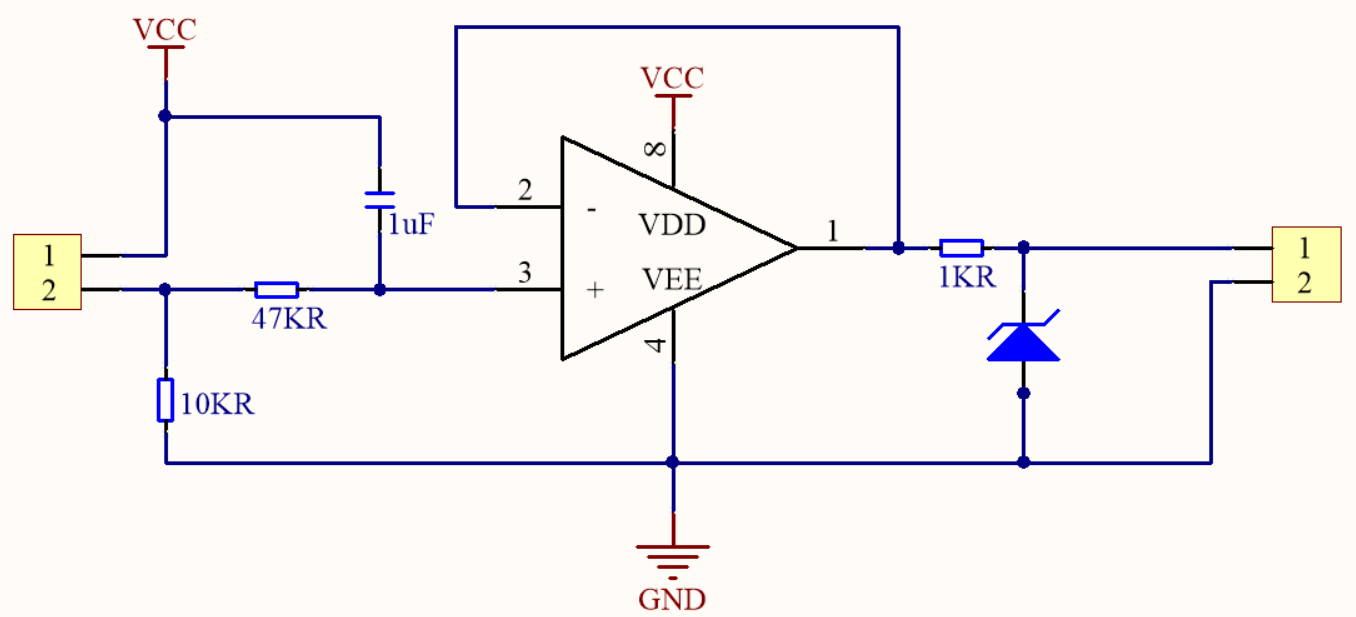
\includegraphics[width=0.65\columnwidth]{images/pcbs/SensorPCB-Switch.png}
    
    \par\end{centering}

    \label{fig:Esquematico-sensor-switch}
\end{figure}

% Referencia para boas práticas de projeto?

Para o roteamento de trilhas na placa, a organização foi realizada
em duas camadas,
agrupando componentes parte do mesmo circuito de maneira próxima, 
tentando seguir boas práticas no projeto de placas de circuito impresso.
Uma visão geral da placa, com todos os componentes montados está 
disponível na figura \ref{fig:Placa-sensoriamento}. Para a geração dos circuitos
e placas, foi utilizado o \textit{software Altium Designer}.
 
\begin{figure}[ht]

    \caption{Placa de sensoriamento.}    
    
    \begin{centering}
    \begin{floatrow}

    \subfloat[Visão 3D com componentes]{
        \begin{minipage}{.5\textwidth}
            \centering
            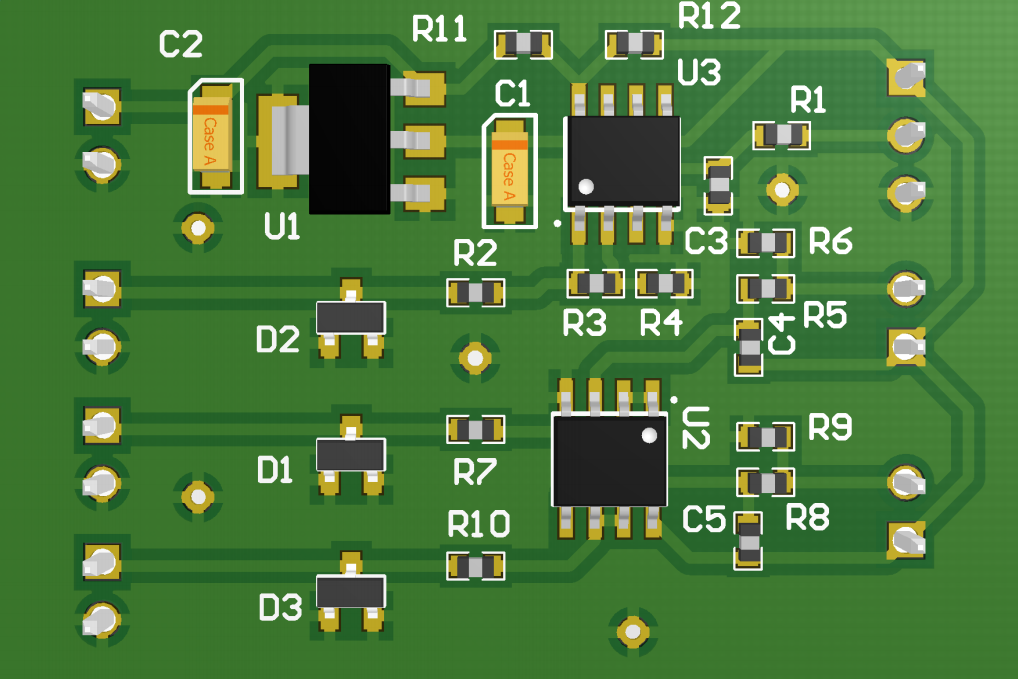
\includegraphics[width=0.9\columnwidth]{images/pcbs/SensorPCB-Board.png}
        \end{minipage}
    }
    
    \subfloat[Visão das trilhas]{
        \begin{minipage}{.5\textwidth}
            \centering
            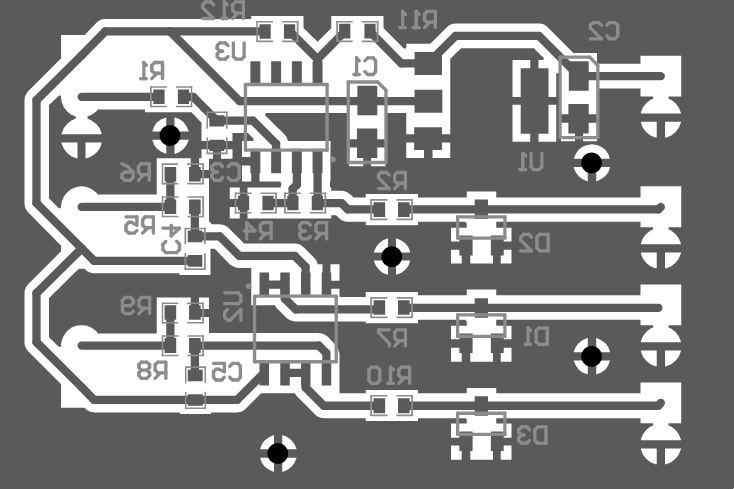
\includegraphics[width=0.9\columnwidth]{images/pcbs/SensorPCB-Board2.png}
        \end{minipage}
    }
    
    \end{floatrow}

    \par\end{centering}

    \label{fig:Placa-sensoriamento}
\end{figure}

\section{Placa de comando}

A placa de comando será aquela responsável por conectar todos os 
componentes do sistema elétrico, de modo a permitir que o 
microcontrolador empregado tenha acesso a todos os periféricos.
Optou-se por posicionar esta placa na base do manipulador, facilitando 
o acesso a esta e sua posição relativa à bateria do sistema.
Para o tamanho da placa, adotou-se que esta poderia ter dimensões semelhantes
às da base, disponíveis na figura \ref{fig:TamanhoPCB-Junta1}.
Foram adotadas então as dimensões de 100x75mm.

\begin{figure}[h]
    \caption{Espaço disponível para inclusão de placa na junta 1}    
    \begin{centering}

        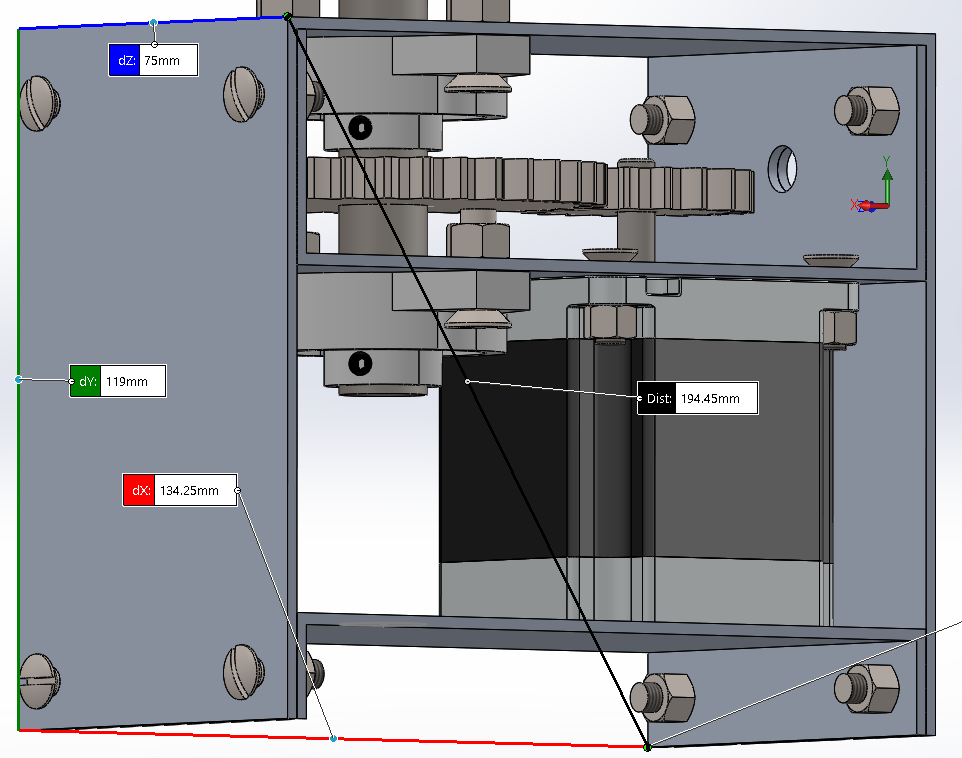
\includegraphics[width=0.7\columnwidth]{images/pcbs/MainPCB-Dimensoes.png}
    
    \par\end{centering}

    \label{fig:TamanhoPCB-Junta1}
\end{figure}

Em relação à alimentação da placa, a tensão de 12V proveniente da bateria será
ramificada para dois pontos distintos: O próprio conector \textit{jack}
do arduino e um conector do tipo borne na lateral da placa.
Ao alimentar a placa através do arduino Mega, faz-se uso do seu 
regulador de tensão interno para geração dos pontos de tensão 5V na 
placa, que juntamente com o pino \textit{Vin}, que é uma extensão do 
sinal 12V na entrada, fornecerão a alimentação para os equipamentos de 
baixa potência. 
O segundo ponto de alimentação servirá para alimentar os motores de 
passo, onde o envio do sinal ao motor é comandado por seu respectivo 
circuito de acionamento integrado.

Os sinais advindos dos sensores fim-de-curso são inicialmente enviados
a um optoacoplador, desse modo, evita-se a propagação de erros resultantes 
de interferência de modo comum nos cabos de transporte e é garantido 
o isolamento elétrico entre as placas do sistema, em relação à essa 
interface.

Na figura \ref{fig:MainPCB-Optoacopladores} é possível ver o circuito
utilizado para transporte do sinal via optoacoplador. O resistor de entrada 
para o diodo emissor de radiação infravermelho foi escolhido atentando-se 
ao valor máximo para a corrente contínua direta de passagem, definida
pelo fabricante no valor de 50mA, valor disposto no \textit{datasheet} do dispositivo PC817C. 
Com uma queda de tensão típica de 1.2V,
e um valor limite de 12V recebido através do conector, o valor mínimo
da resistência pode ser definido como $216\Omega$, seguindo a equação \ref{eq:opto1}.
Buscando uma proteção maior ainda, o valor do resistor foi definido como $2,7k\Omega$, 
limitando a potencia consumida no resistor a 0.0432W.
Neste caso, mesmo com uma tensão de entrada de 5V, como esperado em funcionamento
normal, a corrente direta seria mantida em níveis seguros de utilização,
próximo a 1.4mA.

\begin{figure}[h]
    \caption{Circuito de tratamento dos sinais de fim-de-curso na placa de comando.}    
    \begin{centering}

        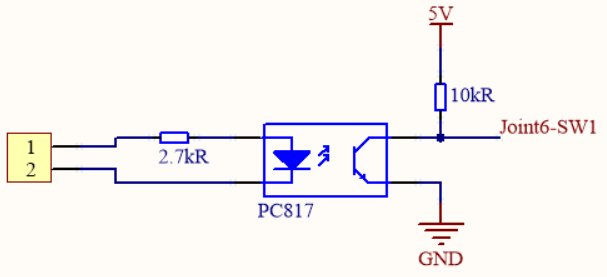
\includegraphics[width=0.65\columnwidth]{images/pcbs/MainPCB-Opto.png}
    
    \par\end{centering}

    \label{fig:MainPCB-Optoacopladores}
\end{figure}

O valor do resistor na saída do circuito deve ser 
escolhido de modo que seja observada uma queda de tensão suficiente 
para que o valor lido na saída seja pequeno o suficiente para garantir
um nível de leitura correto pelo controlador, assim, foi definido que a 
queda de tensão deve ser igual a 5V. A corrente de entrada mantém-se 
entre 1mA e 4mA para valores entre 5V e 12V na entrada, o que equivale
a um ganho do optoacoplador entre 70\% e 120\%, como pode ser visto no 
gráfico da figura \ref{fig:opto-CTR}, retirado da ficha catalográfica do 
dispositivo PC817C. 
Assumindo a configuração que forneça a menor corrente na saída, 1mA e 70\%, a corrente resultante
atinge o valor de 0,7mA, logo, o valor mínimo de resistência na saída 
para uma queda de tensão de 5V deve ser de aproximadamente $7,1k\Omega$, optando-se então pelo valor 10k$\Omega$,
para atribuir maior confiabilidade ao circuito.

\begin{figure}[h]
    \caption{Gráfico relacionando CTR com corrente de entrada para dispostiivos PC817C.}    
    \begin{centering}

        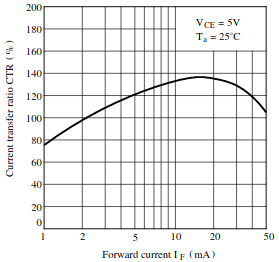
\includegraphics[width=0.5\columnwidth]{images/pcbs/opto-CTR.png}
    
    \par\end{centering}

    \label{fig:opto-CTR}
\end{figure}

Para a leitura dos dados analógicos dos potenciômetros,
inicialmente foi pensado em utilizar amplificadores de instrumentação,
a fim de, assim como no caso dos sensores fim-de-curso, garantir uma 
robustez em relação a interferências de modo comum e isolar os dois 
pontos do sinal. Contudo, observou-se que amplificadores de 
instrumentação poderiam encarecer razoavelmente o projeto, logo, esta alternativa foi 
descartada.
Outra opção seria implementar um amplificador de instrumentação 
utilizando amplificadores comuns, mas para obter resultados de 
amplificação decentes o circuito dependeria da escolha de componentes
semelhantes, ocorrendo então uma incerteza relativa ao equilíbrio do 
valor de resistências, que poderiam acarretar em erros na amplificação, 
portanto, esta alternativa também foi rejeitada.

Optou-se então pela saída mais simples, conectar um dos terminais do 
sinal do potenciômetro ao terra do circuito e enviar o outro a um 
amplificador na configuração de seguidor de tensão, garantindo o 
isolamento desejado e alta impedância de entrada para leitura do sinal.
Adotou-se então que o sinal deverá ser transportado por par de cabos
trançados e blindado, minimizando os efeitos de interferências.

A figura \ref{fig:MainPCB-Pot} demonstra o circuito utilizado para uma 
única junta, como serão utilizados 3 potenciômetros, decidiu-se por 
empregar um componente que tenha no mínimo 3 amplificadores no mesmo 
circuito integrado, a exemplo do LM324, que ainda possui características
como possibilidade de operação em \textit{single-supply} e baixa corrente
de \textit{bias}.

\begin{figure}[h]
    \caption{Circuito de tratamento dos sinais de potenciômetros na placa de comando.}    
    \begin{centering}

        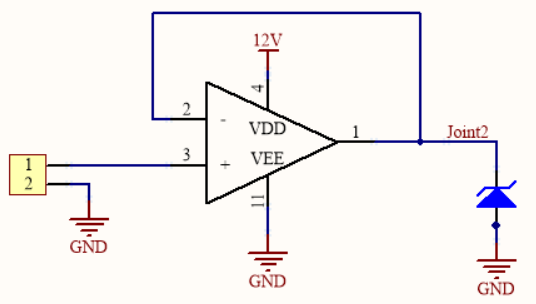
\includegraphics[width=0.6\columnwidth]{images/pcbs/MainPCB-Pot.png}
    
    \par\end{centering}

    \label{fig:MainPCB-Pot}
\end{figure}

Para acionamento dos motores DC, os únicos dispositivos empregados foram
resistores de terminação para os sinais PWM a serem enviados, na tentativa de igualar
a impedância do emissor do sinal com a impedância da linha, 
evitando efeitos indesejados, como reflexão de sinal e redução
da integridade do sinal de acionamento. Os dispositivos escolhidos para
comandar os motores DC possuem na entrada um \textit{buffer/line driver},
evitando perda excessiva de potência do sinal de comando e inserindo uma 
proteção nos circuitos envolvidos, referente ao isolamento dos sinais.

Em relação aos motores de passo foram também empregados resistores de 
terminação para os sinais de \textit{enable}, direção e passo, buscando 
maior integridade do sinal na própria placa. Os sinais de \textit{reset}
e \textit{sleep} foram conectados entre si e à trilha de 5V por um 
resistor do tipo \textit{jumper}. O sinal de \textit{fault} também 
foi conectado à trilha de 5V por um resistor de $0\Omega$. Essas conexões
permitem que outros tipos de dispositivos de acionamento integrado sejam conectados à placa,
como por exemplo o A4988, evitando dependências do circuito a um tipo específico de
controlador. 
Seguindo a recomendação do fabricante, exposta na ficha catalográfica do dispositivo, 
foi adicionado, para cada CI, um capacitor eletrolítico no valor
de 100uF entre o pino de alimentação do motor e o sinal de referência
do circuito.   

O valor escolhido para os resistores de terminação é simbólico,
sendo que uma vez que a manufatura das placas e barramentos de comunicação
estejam finalizados, o correto valor deverá ser definido através de 
testes da impedância da trilha e do cabo equivalentes.

Os circuitos de acionamento dos motores estão dispostos na figura \ref{fig:MainPCB-Motors}.

\begin{figure}[h]

    \caption{Circuito de acionamento para os diferentes tipos de motores}    
    
    \begin{centering}
    \begin{floatrow}

    \subfloat{
        \begin{minipage}{.3\textwidth}
            \centering
            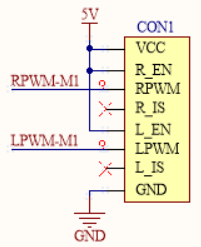
\includegraphics[width=0.7\columnwidth]{images/pcbs/MainPCB-DCmotor.png}
        \end{minipage}
    }
    
    \subfloat{
        \begin{minipage}{.7\textwidth}
            \centering
            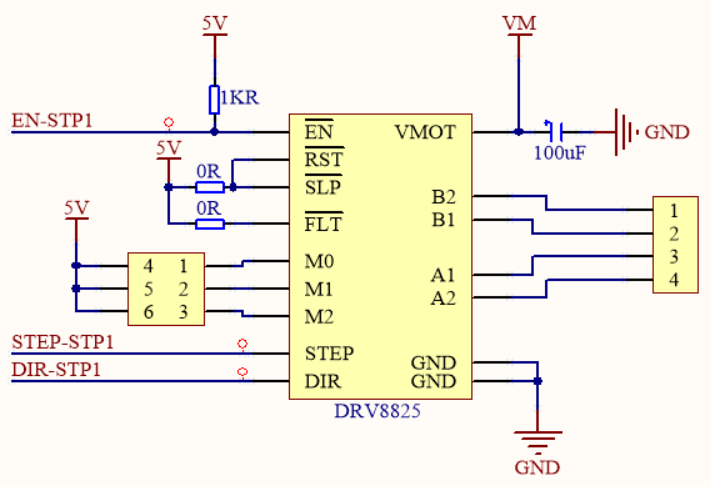
\includegraphics[width=0.8\columnwidth]{images/pcbs/MainPCB-Steppermotor.png}
        \end{minipage}
    }
    
    \end{floatrow}

    \par\end{centering}

    \label{fig:MainPCB-Motors}
\end{figure}

Pela figura \ref{fig:MainPCB-Motors} nota-se um resistor com a 
função de \textit{pull-up} no pino de \textit{enable} dos circuitos integrados de acionamento
dos motores de passo, para garantir que estes não serão ativados a menos que devidamente 
configurados pelo microcontrolador. Nota-se também uma conexão entre 
os pinos de definição da resolução do passo dos motores de passo e o 
sinal de 5V, para que a resolução do passo possa ser pré-definida via
\textit{hardware}.

Foram incluídos também na placa circuitos para tratamento dos sensores 
do \textit{joystick} para interfaceamento com o usuário, contando 
com amplificadores para tratamento dos sinais analógicos, terminal para
interface com efetuador final, botão de \textit{reset} e circuito para
conexão com possível botão de segurança.

Como dito anteriormente, o arduino Mega possui 54 pinos para comunicação
digital, dos quais 15 apresentam funcionalidade PWM e 6 podem funcionar
como fontes de interrupção externa. Os diversos sinais da placa foram 
organizados de modo a facilitar o controle futuro, velocidade de resposta
na leitura dos sensores e facilitar o roteamento de trilhas na placa. 
Seguindo estas heurísticas, chegou-se à organização descrita na tabela
\ref{tab:Pinout}.

\begin{table}[h]
    \begin{centering}

    \begin{floatrow}

    \subfloat{
        \begin{tabular}{|c|c|}
            \hline
            Funcionalidade & I/O Arduino \tabularnewline
            \hline
            \hline
            Junta 1 - Fim-de-curso & D11 e D12 \tabularnewline
            \hline
            Junta 2 - Fim-de-curso & D21 e D20 \tabularnewline
            \hline                
            Junta 3 - Fim-de-curso & D19 e D18 \tabularnewline
            \hline
            Junta 4 - Fim-de-curso & D10 e D50 \tabularnewline
            \hline
            Junta 5 - Fim-de-curso & D51 e D52 \tabularnewline
            \hline
            Junta 6 - Fim-de-curso & D53       \tabularnewline
            \hline                                   
            Joystick (X/Y/Z) & A1/A0/D3 \tabularnewline
            \hline     
            Botão segurança & D2 \tabularnewline
            \hline        
            Efetuador final - PWM & D13 \tabularnewline
            \hline   
        \end{tabular}
    }

    \subfloat{
        \begin{tabular}{|c|c|}
            \hline
            Funcionalidade & I/O Arduino \tabularnewline
            \hline
            \hline
            Junta 1 - EN/DIR/STP & D30/D32/D45 \tabularnewline
            \hline
            Junta 2 - PWM L/R & D8 / D9 \tabularnewline
            \hline
            Junta 3 - PWM L/R & D6 / D7 \tabularnewline
            \hline                
            Junta 4 - PWM L/R & D4 / D5 \tabularnewline
            \hline
            Junta 5 - EN/DIR/STP & D26/D28/D44 \tabularnewline
            \hline
            Junta 6 - EN/DIR/STP & D22/D24/D46 \tabularnewline
            \hline
            Junta 2 - Potenciômetro & A2       \tabularnewline
            \hline
            Junta 3 - Potenciômetro & A3       \tabularnewline
            \hline
            Junta 4 - Potenciômetro & A4       \tabularnewline
            \hline                                               
        \end{tabular}
    }

    \end{floatrow}

\caption{Organização das conexões dos periféricos à placa central.}
\label{tab:Pinout}

\par\end{centering}
\end{table}

Em relação aos sensores fim-de-curso, nota-se pela tabela \ref{tab:Pinout}
que eles estão posicionados de forma não contínua, esta decisão foi tomada
pautada principalmente no fato de que as portas escolhidas apresentam
possibilidade de geração de interrupção. Os pinos D12, D11, D10, D50, D51,
D52 e D53 podem ser configurados como PCINT6:0, podendo lançar interrupção
ao ser detectada variação em qualquer uma dessas entradas, já os pinos
D21, D20, D19 e D18 estão ligados diretamente a fontes de interrupção
própria. O lançamento de interrupção garante uma rápida resposta
do sistema ao atingir algum ponto limite em alguma junta. O botão de 
segurança e eixo-z do \textit{joystick} foram semelhantemente conectados
a fontes de interrupção, a fim de garantir facilidade e rapidez na leitura desses
valores.

Outra escolha foi a conexão dos pinos de comando de passo (STP) dos
motores de passo a pinos do microcontrolador atmel2560 que possuem
funcionalidades PWM, desse modo, a funcionalidade PWM pode ser alterada
para avanço dos motores. 
As demais conexões foram realizadas tomando como base principalmente 
a facilidade no roteamento das trilhas na placa.

No que diz respeito ao roteamento e organização dos sinais na placa, 
a prioridade inicial foi em manter trilhas pequenas, reduzindo a 
interferências entre sinais na placa, em seguida, buscou-se manter 
circuitos com funcionalidades semelhantes e/ou relacionadas agrupados
entre si.

A figura \ref{fig:Placa-controle} demonstra o estado final da placa 
após o roteamento de todas as trilhas necessárias para o comando.
Nota-se que os sinais dos motores e sinais de leitura dos potenciômetros
estão agrupados de forma simples e intuitiva, no entanto, os sinais de 
leitura dos sensores fim-de-curso foram dividos em 3 locais da placa, 
isto ocorreu pois os pinos de conexão escolhidos para leitura desses 
sinais são fisicamente distantes na própria placa do arduino. Em 
relação ao conector do \textit{joystick}, pelo fato das entradas análogicas e 
pino de interrupção selecionado estarem em lados distintos da placa, o
sinal do eixo-z foi separado e aproximado de sua entrada digital.

\begin{figure}[ht]

    \caption{Placa de comando.}    
    
    \begin{centering}

    \subfloat[Visão 3D com componentes]{
        \begin{minipage}{1\textwidth}
            \centering
            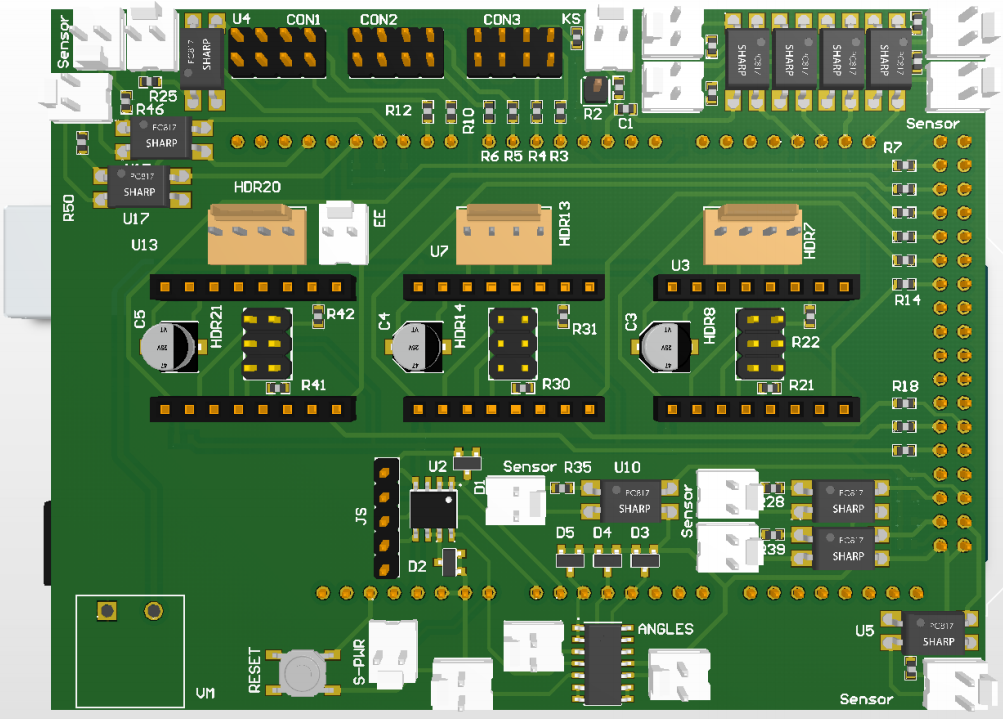
\includegraphics[width=0.9\columnwidth]{images/pcbs/MainPCB-Board.png}
        \end{minipage}
    }
    
    \subfloat[Visão das trilhas]{
        \begin{minipage}{1\textwidth}
            \centering
            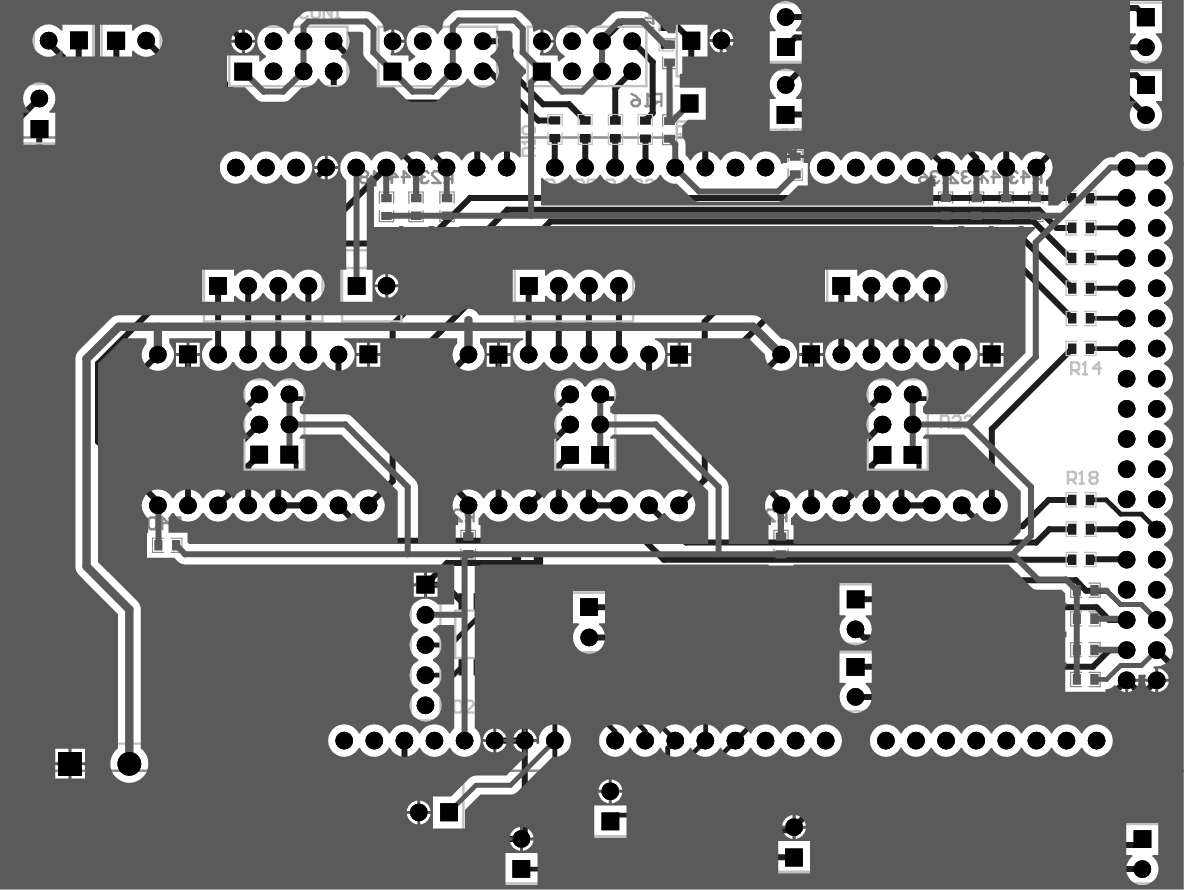
\includegraphics[width=0.9\columnwidth]{images/pcbs/MainPCB-Board2.png}
        \end{minipage}
    }

    \par\end{centering}

    \label{fig:Placa-controle}
\end{figure}